\chapter{Trusted computing}
Nowadays, the modern computing system is made up of many highly
distributed components.

Let's take into consideration the typical distributed infrastructure,
it's made up of a cloud for storage and computation, which communicate
with other devices outside its cluster, such as IoT devices, via edge
routers. Securing all those components it's a real challenge, because
each of those devices could be different, as well as their
communication technologies(Wired, Wireless, etc.). 

While in the past we had physical components, nowadays the trend is
\textbf{softwarization of the components} on top of a generic
commodity hardware, with "tools" such as SDN, NVF, etc.
\begin{boxH}
  As a consequence, systems \textbf{more flexible} but \textbf{more
  vulnerable}.
\end{boxH}
After all, the larger the software base, the higher the probability of
bugs, especially in the software, but hardware bugs are to be taken 
into consideration as well. All this without even considering the
issue of software updates

One of the main issues nowadays is \textbf{trustworthiness}, that being if
something behaves exactly as expected. However, there are several problems
related to trust in this context:

\begin{itemize}
    \item Trust in the cloud provider(s)
    \item Trust in the network/edge provider(s)
    \item Low or no access control for edge- and end-devices
    \item Low-cost IoT devices (which typically imply low security)
    \item Personal devices (often managed by users with limited 
          security knowledge)
\end{itemize}

If possible, it is recommended to protect the infrastructure by
avoiding or blocking all the possible attacks, which is a basically
impossible task. If protection is not feasible, one should do the next
best thing, that being monitoring the state of the system for early
detection and reaction to attacks. IDS can help to this end, but they
can be eluded by the attacker, so the best solution is to provide 
\textbf{integrity verification}, meaning that the system has not been
tampered with, both of the software component as well as their
configuration.

Integrity concerns can be categorized into hardware and 
software aspects:

\begin{itemize}
  \item \textbf{Hardware:}
    \begin{itemize}
      \item Am I communicating with the correct (intended) node?
      \item Does it host the expected (physical) components? For this
        reason, each contry is developing their own components
    \end{itemize}
  \item \textbf{Software:}
    \begin{itemize}
      \item Am I communicating with the correct (intended) 
        software component?
      \item Is it correctly configured?
      \item Is the baseline software the expected one?
    \end{itemize}
\end{itemize}

As we just explained, trust is a big issue in modern computing, and 
in order to answer all those questions, we need to consider some
solutions.
\section{Trusted Execution Environment (TEE)}
Systems are complex, and its difficult to trust every single
component, but we can create a small environment that we can trust.
But first, let's give again a definition of what trust is.
\begin{boxH}
  Something sor someone is \textbf{trusted} if one can \textbf{rely}
  upon to \textbf{not compromise your security}, without any
  guarantees.
\end{boxH}

Similarly, something is \textbf{trustworthy} if it \textbf{will not
compromise your security}, thinking about whether it is safe to use
something or not.

If something is trustworthy it is trusted, but not vice versa.

Trusted Execution Environment is what you may choose to rely upon to
execute sensitive tasks, which are called \textbf{Trusted
Applications} (TA), and which one hope to be trustworthy. 

TEE were originally developer for smartphones, which made them
necessary due to the high number of apps running on the same
environment, some of those with critical data(CC numbers, etc.), but
nowadays they are used in a variety of devices.

\begin{figure}[H]
  \centering
  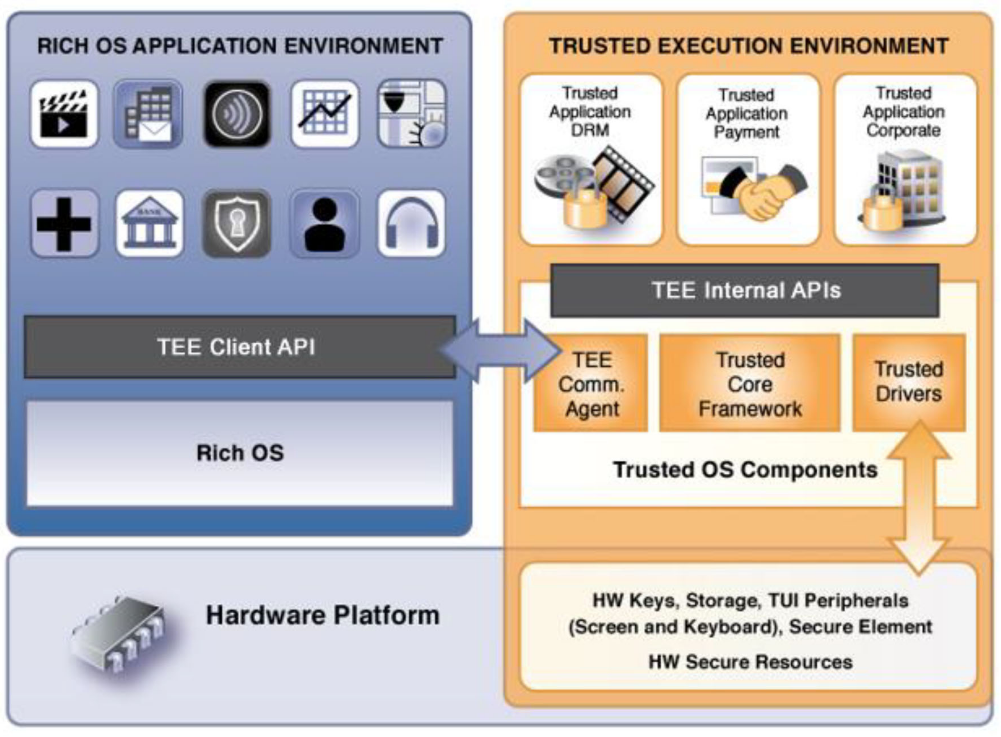
\includegraphics[width=0.5\textwidth]{img/Tee and REE.png}
  \label{fig:tee and ree}
  \caption{Trusted Execution Environment and Rich Execution
  Environment}
\end{figure}

As you can see from figure \ref{fig:tee and ree}, one one device can
run different enviroments at the same time On of those is a
\textbf{Rich Execution Environment} (REE), which is the normal
environment in which one runs any applications or OS. On the other
hand, the TEE is a separate environment isolated from the rest of the
system to run critical tasks and has access to some trusted ankles
like the hwardware keys, the secure storage, peripherals, etc.
TEE can only run on some specific hardware platform made up of trusted
components(not trustworthy, but trusted): the trusted drivers, the
core framework(the execution core) and a set of API accessible only
from trusted applications, the TEE communication agent 

In modern computing, TEE has become an important subject, especially
in the field of "confidential computing," which is actively promoted
by the Confidential Computing Consortium (CCC). The primary goal of
TEE is to protect "data in use," ensuring that nobody else can read or
write the data. Only authorized applications are allowed to process
the data. This approach contrasts with various cryptographic
techniques used to protect "data at rest" and "data in motion."

A key component of TEE, necessary to provide it's services, is the
\textbf{Root of Trust} (RoT), which is an element whose misbehavior
cannot be detected during runtime. The RoT must be \textbf{both
trusted and trustworthy}. It is also part of the Trusted Computing
Base (TCB), which is the set of hardware, firmware, and software
components critical to the system's security. Any vulnerability within
the TCB poses a significant threat to the system’s overall security.

\subsection{TEE Security Principles}

The security principles of a Trusted Execution Environment 
(TEE) involve the following:

\begin{itemize}
    \item Being part of the device's secure boot chain (based on a Root 
    of Trust) and verifying code integrity during each device boot.
    \item Hardware-based isolation from the device’s rich OS 
    environment to execute sensitive code.
    \item Isolation of Trusted Applications (TAs) from each other.
    \item Secure data storage, using a hardware-unique key accessible 
    only by the TEE OS to prevent unauthorized access, modification, 
    and any possibility of data exploitation on other devices.
    \item Privileged and secure access to peripherals (trusted path).
    \item Hardware isolation of peripherals (e.g., fingerprint sensors, 
    displays, touchpads) from the rich OS environment, controlled 
    only by the TEE during specific actions, with no visibility or 
    access by the Rich Execution Environment (REE), including 
    malware.
\end{itemize}

\section{Some TEE Implementations}
\subsection{Intel Identity Protection Technology (Intel IPT)}

Intel Identity Protection Technology (Intel IPT) is a security feature
that operates on a dual-CPU system within Intel processors. This
design leverages the Management Engine (ME), a dedicated CPU that
exists alongside the primary CPU in Intel processors. While the
primary CPU executes user tasks, the ME, integrated into the chipset,
can perform various management and security functions independently.
Typically, the ME is unused in consumer devices, but in corporate
environments, it can be activated even when the device is off via
features like wake-on-LAN, allowing remote management over Wi-Fi or
Ethernet.

Intel IPT uses the ME to run a \textbf{Java applet} isolated from the
main CPU, offering enhanced security for tasks such as cryptographic
key generation and storage, which integrates seamlessly with the
Windows Cryptographic API. Additionally, Intel IPT supports secure
One-Time Password (OTP) generation, as seen in applications like
VASCO's MYDIGIPASS.COM, which use the ME to securely store secrets for
OTPs. Another significant feature is secure PIN entry, where the
chipset manages video output to ensure the security of PIN input by
isolating it from the main system.

The ME's integration into the hardware, running on separate CPU
architecture, exemplifies a physically separated Trusted Execution
Environment (TEE), offering distinct security advantages by isolating
critical operations from the main processing tasks.

\subsection{ARM TrustZone}

ARM TrustZone is a Trusted Execution Environment (TEE) implemented in
certain ARM CPUs, designed to provide a secure and a normal mode
within the same processor. To achieve this, TrustZone extends the
CPU's bus with an additional "33rd bit" that signals whether the
processor is in secure or normal mode. This signal is exposed outside
the CPU, which enables secure peripherals and secure RAM by allowing
the system designer to control access to memory and devices based on
the security mode.

While the TrustZone framework is open and well-documented, it has some
limitations. TrustZone can only support a single secure enclave at a
time, and this security relies on software-based separation between
applications rather than on distinct hardware boundaries, making it
somewhat less secure than fully hardware-isolated environments. ARM is
actively working to expand TrustZone by introducing a third
operational mode to accommodate specific features like attestation.
However, adding this capability presents challenges due to backward
compatibility concerns, as ARM aims to preserve the success of its
platform without disrupting existing applications.

\subsection{Trustonic}

The main issue with TrustZone is that it only one secure enclave. 
To address this issue, Gemalto developed the Trusted Foundations 
system, and Giesecke+Devrient (G+D) created MobiCore. 
Both solutions effectively divide the single secure enclave into 
multiple enclaves by leveraging a smart-card operating system. 
Trustonic’s development is based on MobiCore, requiring 
license fees for implementing the code. Trustonic's TEE OS, 
named "Kinibi," includes enhancements such as version 500, 
which supports 64-bit Symmetric Multiprocessing (SMP) for 
embedded systems. Samsung Knox presents a similar approach 
but additionally incorporates secure boot functionality.

\subsection{Intel SGX}

Intel Software Guard Extensions (SGX) are tightly integrated with the
CPU, providing a hardware-based TEE by modifying memory management to
enhance security. SGX enables the creation of secure enclaves, which
are isolated execution environments protected from access by other
processes, even those with high priority. These enclaves achieve
memory isolation, ensuring that only the code within an enclave can
access its data, providing a high level of hardware-protected
separation.

When an SGX enclave is created, the Intel SGX architecture performs a
measurement, similar to Trusted Platform Module (TPM) practices, by
computing a hash of the executable loaded into the enclave. This
measurement-based security model is essential to SGX’s integrity,
ensuring that only approved code can run within an enclave.

For extended capabilities, SGX can be paired with Intel Identity
Protection Technology (IPT), allowing features such as a trusted
display. However, SGX itself is limited to CPU and memory protection
and does not provide secure input/output channels. When trusted
input-output is required, pairing with Intel IPT enables trusted
interaction with the display.

Intel initially made SGX-1 available across both consumer and
enterprise CPUs, but later revisions—specifically SGX-2—shifted focus
towards server-oriented environments. SGX-2 is now mainly available on
high-end CPUs, such as Intel’s Xeon series, used in data centers.
Furthermore, enclave creation within SGX requires special permissions
and the use of Intel-specific libraries, and all enclave-bound code
must be signed by Intel. This signing requirement means executable
code must be submitted to Intel to receive a signature, which may be a
barrier for some users.

\subsection{Keystone}

Keystone is an open-source framework designed for building Trusted
Execution Environments (TEEs). It allows developers to select only the
necessary features, which helps minimize the Trusted Computing Base
(TCB), because smaller the trust "surface" the better. The
architecture consists of an untrusted environment, such as a
general-purpose operating system, combined with multiple trusted and
segregated enclaves. Keystone is built on top of RISC-V, which offers
customizable open-source hardware options, including
Field-Programmable Gate Arrays (FPGAs) or System-on-Chip (SoC)
designs. The framework incorporates core components along with
cryptographic extensions and supports various execution modes,
including Machine(M), Supervisor(S), and User(U) modes. Additionally, it
features Physical Memory Protection (PMP), which has its
hardware-based access control to different pages of memory. That
avoids that one process can access the memory of another process,
either in general or specifically during a period of time. This helps
to safeguard memory and I/O operations, which are memory mapped.

Usually, TEEs are rigid and un-customizable, with many design
implementation dictated from the underlying hardware, for example
Intel SGX has a large software stack that is not customizable which
means a larger TCB, which is undesirable, AMD SEV
have the same issue and ARM TrustZone has a single TEE. 

The architecture is shown in figure \ref{fig:keystone}. Keystone is
structured to have a \textbf{Security Monition} as the only program
running in Machine mode(the highest privilege mode), which provides
which provides access control between any call coming from the upper
layers towards the hardware. It also provides an \textbf{untrusted
domain} where one can run any OS compatible with the RISC-V 
architecture(even Linux), which will run in Supervisor mode. 
Furthermore, to minimize the TCB, no hypervisor or base operating
systems are required.

On the other hand, one can have many \textbf{Enclaves}, which are 
isolated from the untrusted domain and from each other. Since they
dont need a general purpose OS, they run on a \textbf{Keystone 
Runtime}, which is a small OS that provides the necessary services 
to the specific application. On top of this, the \textbf{Keystone 
Application} runs, which is the actual application that the user 
wants to run.

\begin{figure}[H]
  \centering
  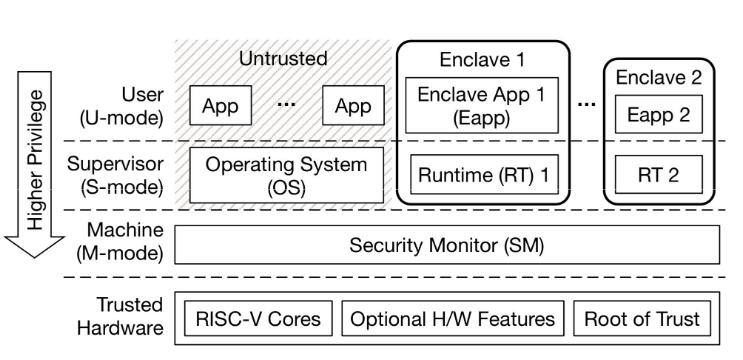
\includegraphics[width=0.6\textwidth]{img/keystone architecture.png}
  \label{fig:keystone}
  \caption{Keystone architecture}
\end{figure}

\begin{boxH}
  For the exam, read the bloody papers.
\end{boxH}

\section{Trusted computing and remote attestation}
Attacker would obviously like to inject malwares at the lowest level
possible, this is to remain undetected while still having access to
the largest part of the system. For this reason the ideal scenario is
to modify the OS is possible, or, alternatively boot an alternative
one under the control of the attacker by modifying the boot sequence
or even the bootloader.

It comes natural after this that the boot system and the OS should be
protected in order to trust the system: for boot sequencing we once
had the BIOS (Basic Input Output System), developed by specific
hardware vendors(no general purpose one available) which was very
difficult to protect, then we had UEFI (Unified Extensible Firmware
Interface) , which is more secure with native support for firmware
signature and verification. After this has been initialized, the OS
can be verified before activation.

So the manufacturer of the platform will sign the firmware, the UEFI,
and the hardware at boot will verify the signature. IF it fails, the
firmware has been tampered with, and the system will not boot. This
step is necessary to guarantee trust in the loaded OS.

\subsection{Rootkits}
This is the generic name for a tool that allows to have root access to
a machine. Of those, there are many kinds.

\paragraph{Firmware Rootkits} Firmware rootkits function by
overwriting the BIOS/UEFI or other hardware firmware. This allows the
rootkit to start running before the operating system even begins to
load.

\paragraph{Bootkits} Bootkits replace the bootloader of the operating
system, ensuring that the bootkit is loaded first when the node is
booted, which occurs before the OS itself initializes.

\paragraph{Kernel Rootkits} Kernel rootkits manipulate a section of
the OS kernel, enabling them to start automatically whenever the
operating system loads, embedding themselves within the core processes
of the OS.

\paragraph{Driver Rootkits} Driver rootkits disguise themselves as
trusted drivers used by the operating system (e.g., Windows) to
interact with hardware. By mimicking a legitimate driver, these
rootkits gain access to hardware resources while avoiding detection.
Don't confuse drivers rootkits with firmware ones, the firmware is
permanently stored in read-only memory, while drivers are part of the
OS and loaded at boot-time.

\section{Root of trust}
In general, protecting software with software can not always be the
best idea, as it may fail or have bugs. For this reason, we need
hardware support to protect the software.
At this end, we have a \textbf{Root of Trust}, which is a hardware 
component that is trusted to behave as expected, and is the foundation
for the chain of trust. The RoT should be always part of the Trusted
Computing Base because hardware is anyway operated by software or
firmware
\subsection{SW root-of-trust}

An example from HP Enterprise illustrates a method for firmware
self-protection, or software root-of-trust. HP Enterprise machines
implements a designated “signature” region at a small fixed location
within the final BIOS image, which is typically 16MB in size. Keep in
mind that this was developed before UEFI.

During manufacturing, the SHA-256 hash of the custom BIOS regions is
calculated. These regions include static code, BIOS version
information, and microcode, but not the hash itself, as its yet to be
initialized, at its only based on components that will never be
updated. The computed hash is then sent to an HPE signing server,
which returns a signed hash image (32 bytes) that includes the
signature and certificate information. This signed hash image is
stored in the BIOS “signature” region.

On power-up, the early BIOS code calculates a hash from the 
specified valid BIOS regions and verifies the validity of the 
stored “signature” contents. If the calculated hash matches 
the stored hash, the boot process proceeds; otherwise, the 
system halts, preventing further booting.

Of course, this method is not perfect, as it is still software-based 
and can be compromised. For example an attacker could replace the 
chip, which is soldered on the board, with a compromised one, or add
another memory chip on the free region of the board, which code will
be executed after the BIOS but before the OS without the integrity 
protection of the signature.

\subsection{HW root-of-trust}
The mechanism just described tries to verify firmware from the
firmware, but can we do better? Yes, we can use a hardware root of 
trust to verify the firmware. 

A hardware root-of-trust for firmware protection typically includes 
self-verification, where a static portion of the firmware authenticates 
the updatable section. This approach allows for an internal method 
of validating firmware integrity directly within the firmware itself. 
Alternatively, firmware verification can be managed by an external 
chip, offering a secure, independent means of affirming firmware 
authenticity.

For example take a look at figure \ref{fig:hw rot}, which shows a x86
Denverton CPU(which is quite old) and implements a 16MB SPI flash
memory, which stores the BIOS. It presents a multiplexer in front of
it that connects to both the CPU and an external cryptographic
microcontroller which can both use the SPI bus and drive the
multiplexer. So the decision of which chip can use the SPI bus is
taken by the external cryptographic microcontroller, which will verify
the integrity of the BIOS before allowing the CPU to boot.

Upon successful validation, this chip allows the x86 CPU to exit its
reset state; otherwise, the CPU remains in reset, ensuring security,
meaning that the chip is the true hardware root-of-trust.

The external chip may also include a fusing option, allowing a public
key hash, which is smaller than the public key, to be securely fused
and later used to verify the signature of the hash stored in the
BIOS's signature region. This validation process is similar to the
internal BIOS self-integrity check, with the added benefit of relying
on an external chip, making it the true hardware root-of-trust.

\begin{figure}[H]
  \centering
  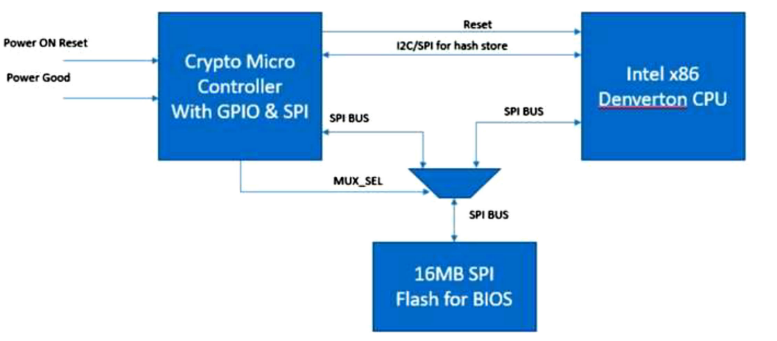
\includegraphics[width=0.6\textwidth]{img/Hw RoT verification.png}
  \label{fig:hw rot}
\end{figure}
\section{Boot Types}
Once we have been able to start the BIOS, the OS can be started.
Different types of boot processes provide varying levels of security
during system startup:

\paragraph{Plain Boot} A plain boot involves no security checks, 
leaving the platform vulnerable to unauthorized modifications.

\paragraph{Secure Boot} In a secure boot process, firmware verifies 
a signature before proceeding. If the verification fails, the platform 
halts, ensuring security from the earliest stages. This process is 
primarily hardware-based and verifies components up to the 
OS-loader.

\paragraph{Trusted Boot} A trusted boot involves the operating system
verifying signatures of critical OS components, such as drivers and
antimalware software. If any verification fails, system operations are
halted. You could have noticed that it assumes that the first part of
the boot up to the firmware was OK and performs verification only of
the operating system components. This type of boot is mainly
software-based and extends verification up to the operational state of
the OS.

\paragraph{Secure boot vs Trusted boot} With secure boot, if the
firmware(BIOS/UEFI/whatever) is compromised, it will not be loaded,
whereas with trusted boot, if the firmware is compromised, the OS
could still be loaded because the firmware is not verified. 


\paragraph{Measured Boot} During a measured boot, the system 
measures each component executed from boot through a defined 
point, denoted as \(X\). Unlike other boot types, measured boot 
does not halt operations if verification fails. Instead, it can securely 
report these measurements to an external verifier, providing 
ongoing insight into system integrity.

What has been just explained is shown in figure \ref{fig:boot types}.
Notice that the trusted drivers and the anti-malware are loaded before
the OS.
% 2 figures 
\begin{figure}[H]
  \centering
  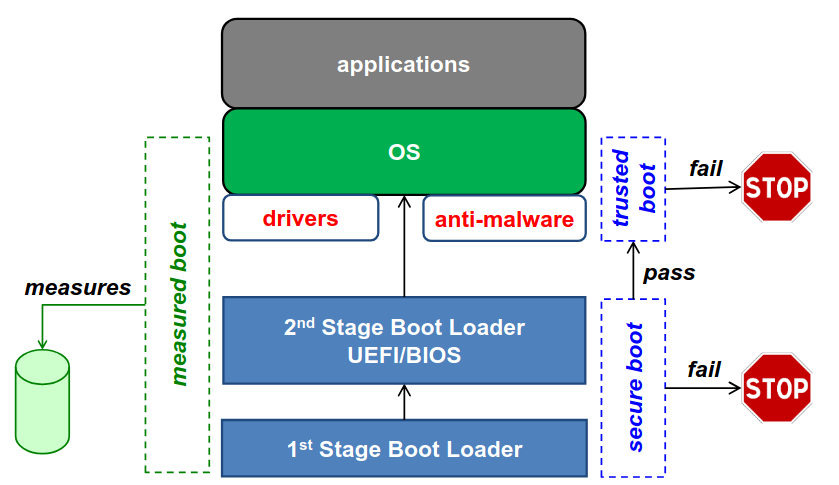
\includegraphics[width=0.6\textwidth]{img/boot types.png}
  \label{fig:boot types}
  \caption{Boot types}
\end{figure}

\subsection*{Windows Boot protection}

Windows 10 and Windows 11 implement a robust boot protection scheme
that combines Secure Boot, Trusted Boot, and Measured Boot to secure
the startup process against malicious interference, as shown in figure
\ref{fig:windows boot protection} . Secure Boot, which is managed by
the hardware manufacturer (e.g., Dell, Lenovo, HP), is the first line
of defense and prevents unauthorized firmware and bootloaders from
running. This step effectively blocks bootkits and ensures that only
trusted firmware initiates the boot sequence.

Following Secure Boot, Windows executes Trusted Boot, which verifies
and loads essential operating system components in a specific order:
first the OS loader, then the kernel, followed by system drivers,
critical system files, and Early Launch Anti-Malware (ELAM) drivers.
ELAM is a fundamental part of anti-malware solutions, as it starts
before any user-space process, offering early protection against
rootkits. The ELAM component must be submitted to Microsoft for
signature to ensure its integrity, enabling a secure foundation for
user-level anti-malware processes to operate later.

In conjunction with Secure Boot and Trusted Boot, Windows also
utilizes Measured Boot, which records each step in the boot process
for verification by an external verifier. If access is granted, this
verifier can query the system to confirm its boot integrity and detect
any potential tampering from the start. This integrated
approach—Secure Boot to lock down firmware, Trusted Boot to load and
verify core OS elements, and Measured Boot to maintain verifiable
logs—creates a strong defense against unauthorized modifications
during the boot process.


\begin{wrapfigure}{r}{0.5\textwidth}
  \centering
  \includegraphics[width=0.5\textwidth]{img/windows boot
  protection.png}
  \label{fig:windows boot protection}
\end{wrapfigure}

\section{Trusted Computing}

Trusted Computing encompasses systems and components designed 
to behave predictably and as expected. In this context, a component 
or platform is considered \textit{trusted} if it consistently performs 
according to predefined expectations, though this does not inherently 
mean it is secure or “good.” Trust in such systems requires verification 
against an expected behavior, rather than an implicit assumption of 
reliability.

A key concept within Trusted Computing is \textit{attestation}, which 
provides verifiable evidence of a platform’s state, allowing assessment 
against a known standard. Another fundamental concept is the 
\textit{Root of Trust}, an inherently trusted component within the 
system that forms the basis for verifying trustworthiness.

Trusted Computing schemes establish trust in a platform by 
identifying its hardware and software components, often through 
a \textit{Trusted Platform Module} (TPM). The TPM plays a crucial 
role in collecting and reporting component identities, offering a way 
to assess hardware and software configurations. This enables 
determination of whether a system’s behavior aligns with expected 
standards, thus supporting the establishment of trust in the platform’s 
integrity.

\subsection{Trusted Computing Base (TCB)}

\begin{boxH}
The Trusted Computing Base (TCB) refers to the \textbf{collection of
system resources}, including both hardware and software, that is
essential in upholding the security policy of a system. 
\end{boxH}

An essential aspect of the TCB is its resilience against compromise;
it must be able to protect itself from threats posed by any hardware
or software outside of the TCB itself.

It is important to note that the TPM \textbf{is not} synonymous with
the TCB of a system. Instead, the TPM serves as a tool for an
independent entity to assess whether the TCB has been compromised. 

In specific implementations, the TPM may also play a preventative
role, ensuring that the system does not start if the TCB fails to
initialize correctly, thus providing an additional layer of security
assurance.

\subsection{Root of Trust (RoT)}

\begin{boxH}
  The RoT refers to a component within a system that must reliably act
  in an expected manner, as any deviation in its behavior cannot be
  detected. 
\end{boxH}

The RoT is essential in establishing trust within a platform
and comprises several foundational components.

The \textbf{Root of Trust for Measurement} (RTM) is responsible for 
taking integrity measurements and transmitting these to the 
\textbf{Root of Trust for Storage} (RTS). Typically, the CPU executes 
the \textbf{Core Root of Trust for Measurement} (CRTM) at boot, 
serving as the first element of BIOS/UEFI code to initiate the 
chain of trust.

The RTS provides a shielded(no one can modify it) and secure storage
environment for critical integrity measurements.
The RTR securely reports the content stored in the RTS, thus enabling
verification of the system's integrity.

\subsection{Chain of Trust}

Our aim is, starting from the lowest level of the firmware, create a
\textbf{chain of trust}.

In a Chain of Trust, each component verifies the integrity of the next
component in sequence. Component A measures Component B and stores
this measurement in the RTS. Then, Component B measures Component C
and similarly stores the measurement in the RTS, continuing this
process down the chain.

Typically, Component A is the CRTM, which is part of the TCB. By using
the \textbf{Root of Trust for Reporting} (RTR), a verifier can
securely retrieve the measurements of Components B and C from the RTS.
For Components B and C to be trusted, Component A must itself be
trustworthy.

\subsection{Trusted Platform Module Overview}

The Trusted Platform Module is an inexpensive component, typically
costing less than 1 dollar, and is available on most servers, laptops,
and PCs. It is designed to be \textbf{tamper-resistant}, although it
is important to note that it is not entirely tamper-proof, meaning
that it is difficult to compromise it, but not impossible.

While the TPM provides security features, it is not a high-speed
cryptographic engine; in fact, it is relatively slow in terms of
processing speed, m.t. doing RSA signatures with it will take forever.
The TPM have to be certified with a \textbf{Common Criteria Evaluation
Assurance Level}(EAL) of 4 or higher, which indicates a certain level
of security assurance, which is quite good indeed.

As a passive component, the TPM requires the CPU to drive its
operations. It does not have the capability to prevent the boot
process; however, it can protect sensitive data and securely report
this information. Consequently, the TPM functions as both the RTS and
the RTR, but it does not serve as the RTM, because we'll perform the
measure and we'll store the results inside the TPM.

The TPM provides secure storage capabilities, functioning as a secure
storage component (RTS) with an extend-only approach. It can report
the content of this secure storage using a digital signature, thus
acting as a reporting entity (RTR). This means that every time that
memory is read outside the TMP, a digital signature computed with a
asymmetric key pair stored inside the TPM is attached to the data.

One of the critical features of the TPM is its hardware random number
generator, which supports various cryptographic algorithms, including
hashing, Message Authentication Code (MAC), and both symmetric and
asymmetric encryption. However, it is important to clarify that the
TPM is not a crypto accelerator, as its performance is relatively
slow.

The TPM also facilitates the secure generation of cryptographic keys
for limited use cases. It supports \textbf{binding}, which encrypts
data using the TPM bind key—a unique RSA key derived from a storage
key. What does that mean? Binding means that if you want to decrypt
this data, you can do that only on the platform that contains that
TPM. Because if you move the data to another platform, they are
encrypted with the key which is not there. This also means that if the
platform broke down, you can't decrypt the data anymore.

Additionally, the TPM allows for \textbf{sealing}, a process
similar to binding, but it also specifies the TPM state required for
the data to be decrypted, or unsealed. This means that the data can be 
decrypted only if the TPM is in a specific state, which is useful to
avoid tampering.

Furthermore, computer programs can utilize a TPM to authenticate
hardware devices. Each TPM chip is manufactured with a unique and
secret \textbf{Endorsement Key} (EK) that is burned in during
production, ensuring that the authenticity of the hardware can be
verified.

\subsection{TPM 1.2}

TPM 1.2 features a fixed set of cryptographic algorithms, which
include SHA-1, RSA, and optionally AES. This version of the TPM
provides a single storage hierarchy specifically for the platform
user, ensuring that key management and storage are centralized.

At the core of TPM 1.2 is a single root key known as the Storage Root
Key (SRK), which is typically an RSA-2048 key. This root key serves as
the foundation for other keys within the TPM, facilitating secure
storage and cryptographic operations.

Additionally, TPM 1.2 incorporates a built-in Endorsement Key (EK)
(RSA-2048) that provides a hardware identity for the platform. This EK
is essential for establishing the authenticity of the TPM and the
device it resides in. 

Another important thing of TPM 1.2 is its capability for sealing
only against the PCRs value, where the measurements are collected. 
\subsection{TPM 1.2}

TPM 1.2 features a fixed set of cryptographic algorithms, which
include SHA-1, RSA, and optionally AES. This version of the TPM
provides a single storage hierarchy specifically for the platform
user, ensuring that key management and storage are centralized.

At the core of TPM 1.2 is a single root key known as the Storage Root
Key (SRK), which is typically an RSA-2048 key. This root key serves as
the foundation for other keys within the TPM, facilitating secure
storage and cryptographic operations.

Additionally, TPM 1.2 incorporates a built-in Endorsement Key (EK)
that provides a hardware identity for the platform. This EK is
essential for establishing the authenticity of the TPM and the device
it resides in. 

Another important feature of TPM 1.2 is its capability for sealing
data to a Platform Configuration Register (PCR) value. This sealing
process ensures that the data can only be decrypted when the platform
is in a specific, verified state, enhancing the security of sensitive
information.
\begin{wrapfigure}{r}{0.5\textwidth}
  \centering
  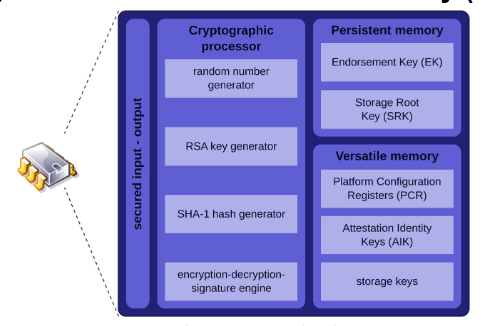
\includegraphics[width=0.5\textwidth]{img/TMP 1-2.png}
  \label{fig:tpm 1.2}
\end{wrapfigure}

\subsection{TPM 2.0}

TPM 2.0 introduces advanced cryptographic flexibility and supports a
range of algorithms, including SHA-1 for backward compatibility,
SHA-256, RSA, ECC-256, HMAC, and AES-128, providing robust options for
secure operations. This version organizes keys into three main
hierarchies: platform, storage, and endorsement. Each hierarchy can
support multiple keys and algorithms, enhancing security management
and allowing for versatile key applications based on specific needs.

A significant feature of TPM 2.0 is policy-based authorization,
enabling more sophisticated and adaptable access controls (in previous
version just one password was required). This policy
framework allows security measures to be tailored according to diverse
requirements and provides a structured way to enforce access
restrictions.

Additionally, TPM 2.0 includes platform-specific specifications
tailored to various application areas, including PC clients, mobile
devices, and automotive environments. Each of these specifications
addresses the unique security requirements of its respective platform,
ensuring that TPM 2.0 can meet the needs of a broad range of use
cases. However, most of the hardware manufacturers implements their
TPMs directly in the CPU or the chipset, meaning that one should check
when buying new hardware: in some cases the TPM is software based on
even virtualized on a dedicated VM thanks to the hypervisor.


\subsubsection{Implementations of TPM 2.0}

TPM 2.0 has several implementation forms, each designed to fit
different hardware and software architectures. The Discrete TPM is a
dedicated chip that implements TPM functionality within its own
tamper-resistant semiconductor package, providing robust security.

In contrast, the Integrated TPM is part of another chip and is not
required to implement tamper resistance. For example, Intel has
integrated TPMs in some of its chipsets, balancing functionality with
space and cost considerations.

The Firmware TPM is a software-only solution that operates within a
CPU's trusted execution environment. Major manufacturers such as AMD,
Intel, and Qualcomm have implemented firmware TPMs, allowing for
flexibility in system design.

Another form is the Hypervisor TPM, which offers a virtual TPM managed
by a hypervisor. This runs in an isolated execution environment and is
comparable to a firmware TPM in terms of security and functionality.

Finally, the Software TPM serves as a software emulator of a TPM,
primarily useful for development purposes. This allows developers to
test and implement TPM functionalities without needing dedicated
hardware.

\subsubsection{TPM 2.0 Three Hierarchies}

TPM 2.0 defines \textbf{three key hierarchies}, each serving distinct
purposes and managing different aspects of security and key storage.

The first hierarchy is the \textbf{Platform Hierarchy}, which is
dedicated to managing the platform’s firmware. This hierarchy utilizes
non-volatile (NV) storage for keys and data, ensuring that critical
firmware-related information is securely maintained.

The second is the \textbf{Endorsement Hierarchy}, which primarily
caters to the privacy administrator. But why we need a privacy admin?
In the early days of the TPM and the Trusted Computing Group (TCG),
there was concern over privacy implications. One issue was that every
time a device’s TPM measured and reported its state, it signed those
measurements with its unique RSA private key. This approach ensured
that the measurements were authentic and uniquely tied to the device,
which was valuable for verifying the integrity of the platform.
However, this method also had a drawback: it revealed the device’s
identity.
If each attestation came from a unique RSA key, it could be traced
back to the same machine each time, compromising privacy.
For this reasons we use different keys for different purposes(key of
the manufacturer, key to identify the owner, \ldots).

Similar to the Platform
Hierarchy, this one also provides storage for keys and data,
emphasizing the importance of privacy in the overall security
architecture.

Lastly, the \textbf{Storage Hierarchy} is designed for the platform’s
owner, who typically also acts as the privacy administrator. This
hierarchy features NV storage for keys and data, allowing for
efficient management of cryptographic assets.

Each of these hierarchies comes with dedicated authorization
mechanisms, such as passwords, and specific policies to govern access
and usage. Additionally, each hierarchy utilizes a unique seed for
generating the primary keys, further enhancing the security and
integrity of the TPM's operations.

\subsection{Using a TPM for Securely Storing Data}

Utilizing a TPM for securely storing data
involves several key considerations to ensure both security and
accessibility.

One primary advantage of using a TPM is its physical isolation. The
storage occurs within the TPM itself, specifically in NVRAM, which
helps safeguard sensitive information. This storage is very small, so
ut usually stores primary keys and permanent keys

To enhance security, Mandatory Access Control (MAC) mechanisms are
employed, which govern how data and keys are accessed within the TPM.
This cryptographic isolation ensures that even if data is stored
outside the TPM, such as on a platform's hard drive, it remains
protected.

When storing keys or data outside the TPM, it is crucial that the
information is encapsulated in a secure format, often referred to as a
blob. This blob must be protected, typically by encrypting it with a
key controlled by the TPM. The use of MAC further reinforces the
security measures, ensuring that access to the stored data is tightly
regulated.

\subsection{TPM Objects}

TPMs utilize various objects to manage cryptographic keys and secure
data. One of the primary types of objects within a TPM is the
\textbf{primary keys}, which includes endorsement keys and storage
keys. These keys are derived from one of the primary seeds stored
within the TPM. Notably, the TPM does not return the private value of
these keys; instead, they can be re-created using the same parameters,
assuming that the primary seed remains unchanged.

In addition to primary keys, TPMs also handle keys and sealed data
objects (SDOs). These objects are protected by a Storage Parent Key
(SPK), which is necessary within the TPM to load or create a key or
SDO. The randomness required for key generation and other
cryptographic functions is provided by the TPM's built-in Random
Number Generator (RNG). 

When a key is generated, the TPM returns the private part, which is
protected by the SPK. However, it is essential to note that this
private part must be stored securely, as its integrity is critical to
maintaining the overall security provided by the TPM.

\subsection{TPM Object Areas}

Trusted Platform Modules (TPMs) categorize the storage structure of
objects into distinct areas, each serving a specific purpose:

\begin{itemize}
  \item \textbf{Public Area:} This area is utilized to uniquely
    identify an object, providing essential information for the
    management of keys and data.

  \item \textbf{Private Area:} Containing the object's secrets, this
    area exists solely within the TPM. It is crucial for maintaining
    the confidentiality and integrity of the keys and data stored
    within the module.

  \item \textbf{Sensitive Area:} This consists of the encrypted
    private area, specifically designed for use when storing sensitive
    data outside of the TPM. It ensures that even when data is not
    housed within the TPM, it remains secure through encryption.
\end{itemize}

\subsection{TPM Platform Configuration Register (PCR)}

The Platform Configuration Register (PCR) serves as the TPM
implementation of Root of Trust for Storage (RTS) and is a core
mechanism for recording platform integrity. PCRs maintain their values
and can only be reset during a platform reset or through a hardware
signal, which ensures that any malicious code cannot manipulate or
retract its measurements.

PCRs are extended using a cumulative hash, following the formula:

\[
\text{PCR}_{\text{new}} = \text{hash}(\text{PCR}_{\text{old}} \, || \, \text{digest\_of\_new\_data})
\]
Basically, the new PCR value is the hash of the old PCR value and the 
new data. This process is repeated for each new piece of data that
needs to be added to the PCR.

This process is commonly referred to as the EXTEND operation (keep in
mind that it's not commutative).
Additionally, PCRs can be utilized to gate access to other TPM
objects. For example, BitLocker uses PCR values to seal disk
encryption keys, ensuring that the keys can only be accessed when the
platform is in a known and trusted state.

\subsection{Measured Boot}

Measured boot builds on secure and trusted boot principles by using
TPM functionality to verify system integrity throughout the boot
process. The key here is that a TPM is available—whether as a separate
chip or firmware module—enabling attestation at each step.

The process begins with the Core Root of Trust for Measurement (CRTM)
located in the boot ROM’s first-stage bootloader. This trusted
component takes the first measurement by capturing the state of the
next component in line, the second-stage bootloader, and stores this
in the TPM’s Platform Configuration Registers (PCRs). This baseline
measurement is critical, as it establishes initial trustworthiness for
everything that comes afterward.

Once the second-stage bootloader is loaded, it continues the process
by measuring the operating system, which can also measure subsequent
applications if needed. The idea is simple: measure each part of the
boot sequence and store these measurements in the PCRs, creating a
chain of trust from the very start.

The accumulated values in the PCRs provide a snapshot of the system’s
integrity, which an external verifier can check to confirm everything
is as expected. Though an internal verifier is possible, an external
one is often more reliable in case an attacker has compromised the
internal components. This setup allows measured boot to act as a
strong line of defense, verifying each stage and ensuring a trusted
environment.

\begin{figure}[H]
  \centering
  \includegraphics[width=0.6\textwidth]{img/Measured boot.png}
  \caption{Measured boot}
\end{figure}
\subsection{Remote attestation procedure}

Remote attestation leverages the values stored in the TPM’s PCRs
during the measured boot process, enabling an external verifier to
confirm the system's integrity. Here’s how it works:

First, an external verifier, which could be a trusted system on the
network, sends a unique challenge (often a nonce) to the device
holding the TPM. This challenge prevents replay attacks by ensuring
that each attestation session is fresh and unpredictable. The platform
then gathers the values of the PCRs requested by the verifier and
packages them along with the challenge.

This package of data—containing the PCR values and the response to the
nonce—is signed using a key unique to the device. This signed response
assures the verifier that it’s seeing legitimate measurements tied to
that specific device.

When the verifier receives the signed package, it performs several
checks:
\begin{enumerate}
  \item \textbf{Signature Validation}: It verifies the signature to
    ensure the data hasn’t been tampered with and is genuinely from the
    device.
  \item \textbf{Identity Validation}: It checks that the device’s
    identity matches expected values, using a stored list of authorized
    machines to confirm that the device is part of the network.
  \item \textbf{Measurement Validation}: Finally, the verifier compares
    the PCR values against known "golden values" stored in a database.
    These golden values reflect the expected configurations for each
    device type—taking into account variations in hardware, firmware,
    and software.
\end{enumerate}

If the PCR values match the golden values, the verifier can
confidently conclude that the system is in a known and trusted state.
If there’s a mismatch, an alert is raised, signaling that the device
may have been compromised or misconfigured.

This remote attestation process provides a robust way to ensure system
integrity across a network by verifying both the software status and
identity of each device, making it a valuable tool for network
security.

\begin{figure}[H]
  \centering
  \includegraphics[width=0.6\textwidth]{img/remote attestation
  procedure.png}
  \caption{Remote attestation procedure}
\end{figure}

\subsection{Management of Remote Attestation}

Remote attestation has been performed, and it has failed. What now?
Management of remote attestation is most important when the
attestation process fails. 

One critical aspect is whether to implement only boot attestation,
which is static, or to include periodic (dynamic) attestation as well.
This decision should take into account the attack model, especially
with respect to runtime vulnerabilities that could be exploited.

The \textbf{periodicity of the attestation} operation is another
important consideration, as it must align with the speed of potential
attacks. A cycle of operations which include the time
required for signature verification, protocol execution, and database
lookups, are typically in the range of several seconds due to the
inherent slowness of TPMs, and for some cases is acceptable, but for
others a window of exposure of even 5 seconds is excessive. 
And that is a limit, not of the attestation, but of the physical
implementation.

Another challenge in remote attestation management is
\textbf{whitelist generation}. This process can be complex in general
but may be less difficult in limited environments, such as Internet of
Things (IoT) devices, edge devices, Software-Defined Networking (SDN),
and Network Function Virtualization (NFV). 

Furthermore, it is essential to label components appropriately—such as
good, old, buggy, or vulnerable—and to include configurations from
sources like Management and Orchestration (MANO) or network management
tools. While generating labels can be straightforward if the data is
file-based, it becomes significantly more challenging when dealing
with memory-based data.
\subsection{TCG PC Client PCR use (architecture)}
According to the Trusted Computing Group for a PC client the PCRs are
used for various purposes:
\begin{wrapfigure}{r}{0.5\textwidth}
  \centering
  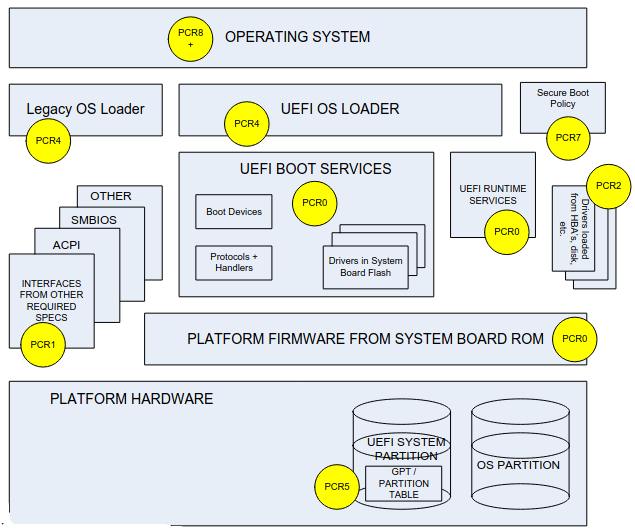
\includegraphics[width=0.5\textwidth]{img/TCG PC Client.png}
  \label{fig:TCG PC Client PCR use}
  \caption{TCG PC Client PCR architecture}
\end{wrapfigure}

\begin{itemize}

  \item PCR0 is measuring the Platform firmware from system board ROM
    and it is a fixed value given one version of the firmware.
    Typically, in a database there are different values for PCR0
    according to the version of the firmware and the version running
    in a device could be deduced by these values. It also stores the
    UEFI boot services, UEFI runtime services.
  \item PCR1 contains the hash of various extensions of the firmware
    (ACPI, SMBIOS, OTHER).
  \item PCR2 drivers loaded from the disk.
  \item PCR3 is not here. That means it's not used for PC.
  \item PCR4 is the part of the UEFI OS loader and of the Legacy OS
    Loader
  \item PCR5 is for the Platform hardware, for example it is reading
    and computing the hash of the partition table. That is important
    if someone manipulated the hardware.
  \item PCR7 contains the Policy for Secure Boot.
  \item All registers from PCR8 to above are given to the OS to decide
    what will be used for.
\end{itemize}
For all the registers up to PCR7 the values can be predicted. They
will depend on the kind of platform, version of the firmware or
driver. These values are in the golden: if there are wrong values in
those registers the system cannot be trusted.
\begin{table}[H]
  \centering
  \begin{tabular}{|p{0.1\textwidth}|p{0.9\textwidth}|}
    \hline
    \textbf{PCR Index} & \textbf{PCR Usage} \\ \hline
    0 & SRTM, BIOS, Host Platform Extensions, Embedded Option ROMs and
    PI Drivers \\ \hline
    1 & Host Platform Configuration \\ \hline
    2 & UEFI driver and application Code \\ \hline
    3 & UEFI driver and application Configuration and Data \\ \hline
    4 & UEFI Boot Manager Code (usually the MBR) and Boot Attempts \\
    \hline
    5 & Boot Manager Code Configuration and Data (for use by the Boot
    Manager Code) and GPT/Partition Table \\ \hline
    6 & Host Platform Manufacturer Specific \\ \hline
    7 & Secure Boot Policy \\ \hline
    8-15 & Defined for use by the Static OS \\ \hline
    16 & Debug \\ \hline
    23 & Application Support \\ \hline
  \end{tabular}
  \caption{PCR Index and Usage}
  \label{table:pcr_usage}
\end{table}

\subsection{Measured Execution}
Previously, we discussed measured boot, which verifies the integrity 
of the system during the boot process. We would like to extend this
functionality to the application that runs on the OS, but to do so we
would have to store the measurements in PCRs, which are limited in 
number.For this reason we can simply use one PCR and extend the
measurements of each application.

Another issue also arises: the value of the PCR depends on the
execution order, in fact starting an application A before an
application B will result in a different value of the PCR than
starting the application B before the application A.
For this reason, the OS can measure the application before loading it
and perform the extend operation of the PCR, but not all OS are able
to do so(the superior OS can).
\subsubsection{Linux’s IMA}

The \textbf{Integrity Measurement Architecture} (IMA) in Linux is a
standard component of the Linux kernel(one needs to enable it)
that extends attestation capabilities to dynamically executed
elements, such as applications. It provides mechanisms for collecting,
storing, appraising, and protecting measurements to ensure the
integrity of files accessed on the system.
It can perform various operations:

\begin{itemize}
  \item \textbf{Collection}: IMA measures a file before it is
    accessed, creating an integrity measurement to track any potential
    alterations.
  \item \textbf{Store}: The measured data is added to a
    kernel-resident list, known as the Measurement List (ML), and the
    IMA PCR (specifically PCR 10) is extended to reflect these
    measurements, making them available for attestation purposes.
  \item \textbf{Appraise} (optional): IMA can enforce local validation
    of a file's measurement by comparing it to a "good" value stored in
    the file's extended attributes. This step helps to ensure that the
    file remains in a trusted state, but is a feature which
    is not required for measured operations
  \item \textbf{Protect} (optional): IMA can secure a file's extended
    security attributes, including the appraisal hash, against offline
    attacks. This prevents unauthorized modifications to these
    attributes when the system is not active.
\end{itemize}
The appraise feature is most interesting: lest's suppose that one
think that, for example, a python executable has been compromised. One
can use an extended attribute to store the hash of the python 
executable and compare it with the hash of the python executable 
measured by the IMA. This happends before it's been executed,
automatically by the OS. If the hashes are different, the python
executable is not executed.

When the IMA starts, it extends UEFI's measured boot concept to the OS
and applications by using PCR 10. It begins by storing a "boot
aggregate," which is a hash of all PCR values from 0 to 7—these PCRs
capture UEFI-related measurements. This boot aggregate establishes a
continuity between the boot measurements and IMA's ongoing monitoring,
preventing certain types of attacks.

IMA is configurable through an "IMA template," which defines what gets
measured. A common template, "IMA-NG," is often used, but the template
can be customized to fit specific needs. IMA then logs these
measurements in the kernel security filesystem, where they’re stored
as ASCII runtime measurements, allowing access to a detailed record of
measured files and executables. For example, each entry includes the
PCR 10 value, a template hash, and hashes for each file, showing the
order in which each executable or library was measured.

\begin{table}[h!]
  \centering
  \begin{tabular}{|c|c|c|c|c|}
    \hline
    \textbf{PCR} & \textbf{template-hash} & \textbf{template} & \textbf{filedata-hash} & \textbf{filename-hint} \\
    \hline
    10 & 91f34b5[...]ab1e127 & ima-ng & sha1:1801e1b[...]4eaf6b3 & boot\_aggregate \\
    10 & 8f16832[...]e86486a & ima-ng & sha256:efdd249[...]b689954 & /init \\
    10 & ed893b1[...]e71e4af & ima-ng & sha256:1fd312a[...]6a6a524 & /usr/lib64/ld-2.16.so \\
    10 & 9051e8e[...]4ca432b & ima-ng & sha256:3d35533[...]efd84b8 & /etc/ld.so.cache \\
    \hline
  \end{tabular}
  \caption{Example of IMA Measurement List}
\end{table}


To verify these measurements, a verifier can request the current PCR
10 value. The machine responds with this value along with the detailed
measurement list. To validate, the verifier starts with a zero value,
incorporates the boot aggregate by combining PCRs 0 through 7, and
then processes each measurement in the order they were originally
extended into PCR 10. This step-by-step verification ensures that the
system's state aligns with expected integrity values.

\begin{listing}
  \centering
  \begin{verbatim}
myPCR10 = 0
myPCR10 = extend(boot_aggregate)

foreach measure M of component C
    if (C not authorized) then raise alarm
    if (M != gold_measure(C)) then raise alarm
    myPCR10 = extend(M)
end foreach

if (myPCR10 == PCR10) OK else raise alarm
  \end{verbatim}
  \caption{IMA verification}
\end{listing}


\subsection{Size and Variability of the TCB}

The TCB is as large as the smallest set of code, hardware, personnel,
and processes necessary to be trusted to meet specific security
requirements. A reliable TCB is essential for achieving a secure
system, as it represents the foundation upon which all security
assurances are built.

To enhance confidence in the TCB, several methods can be applied:
\begin{itemize}
    \item \textbf{Static Verification:} Analyzing the TCB without
      executing it to ensure it behaves as expected.
    \item \textbf{Code Inspection:} Manually examining the TCB code
      for potential vulnerabilities.
    \item \textbf{Testing:} Running the TCB through various scenarios
      to check for security flaws.
    \item \textbf{Formal Methods:} Applying mathematical proofs and
      models to verify the TCB's behavior under different conditions.
\end{itemize}

These methods, however, are often expensive and labor-intensive,
making it essential to minimize the complexity of the TCB. 

\begin{boxH}
A smaller, more streamlined TCB reduces the attack surface, yet
simplification alone is insufficient if variability is not controlled.
\end{boxH}

The TPM aims to establish a reliable TCB via the CRTM. However, the
TCB has become increasingly large and dynamic, making consistency more
difficult to maintain. . For example, two “identical” computational
nodes might report different TCB measurements due to slight variances,
but be completely fine.

\subsection{Dynamic Root of Trust for Measurement}
The solution to the variability and complexity of the TCB is the 
Dynamic Root of Trust for Measurement (DRTM).

It is a technique that establishes a trusted environment on demand by
resetting the CPU and starting measurements from a controlled point,
rather than relying on the entire system boot sequence from BIOS
onward. After all, the secure boot can't be tampered with, so we can
start the measurements after that. 

For that purpose, since TPM version 1.2, some dynamic PCRs were added
from 17 to 23. Those are set to $-1$ at boot(the others are usually
set to 0) and can be reset to $0$ by the OS(this operation is not
allowed for the other PCRs, they can be only reset by hardware resets).

PCR 17 is unique in that it is used specifically by DRTM commands,
ensuring the integrity of this late-launch measurement. By allowing
the TCB to start fresh from a known, controlled point, DRTM enables
flexible and secure initialization of trusted environments.

In any case, whatever is the real operation being executed, they have
the same effect. They disable direct memory access, disable all the
interrupts and disable any debugging mode. That means that the program
executing that special instruction is the only thing being executed in
this moment on this computer, cannot be interrupted, no one else can
have access to the memory and no one else can trace it or modify it
via debug. The purpose is to permit to this program to measure and
then execute the secure loader block.

DRTM leverages special processor commands to initiate a secure
environment. These commands include:
\begin{itemize}
    \item \texttt{SENTER} for Intel's Trusted Execution Technology
      (TXT), which executes the SINIT binary module.
    \item \texttt{SKINIT} for AMD's Secure Virtual Machine (SVM).
\end{itemize}

When either of these commands is executed, all processing on the
platform is temporarily halted. DRTM then:
\begin{itemize}
    \item Hashes the contents of a specified memory region, storing
      this measurement in a dynamic PCR.
    \item Transfers control to a specific memory location, where the
      Secure Loader Block (SLB) is measured and executed. this is also
      called \textbf{Late Launch} because it's not the original launch
      of the system, but it's something that happens after the normal
      launch. This helps in avoiding the problem with the PCR values
      that are incorrect when firmware is updated. And the consequent
      problem with the sealed data.
    \item Disables Direct Memory Access (DMA), interrupts, and
      debugging to secure the environment during this process.
\end{itemize}

One last thing to help understand why firmware updates are a problem 
for sealing.
We have mentioned the fact that sealing is like encryption, but it is
attached, it's related to a specific system state. So imagine that you
have sealed data. Then your system say, okay, I'm performing an
update, firmware update. Now you've got a new bias. Next time that you
start your system, even if that bias is correct, so the measurements
are perfect, the sealing will not work. Because they all, if you want
to unseal, you must have that version because of that was the state.
So it means that now we should seal the data, not against the
firmware, but upon some operational state started after the dynamic
route of trust for measurement was executed. Okay, so it's not only a
problem of not having the correct measures because creating a very big
database, it is of course possible to maintain a lot of measurements.
But sealing is one of the worst thing because sealing requires exactly
the same state.


\subsection{Hypervisor TEE}

The DRTM was designed to facilitate the secure loading of a
hypervisor, such as Xen or VMware ESX, which in turn manages and
isolates VMs. When initialized through DRTM, the TPM can attest to the
integrity of the hypervisor, ensuring it has loaded correctly and
securely. Only after a proper load can TPM-sealed storage be accessed
by the hypervisor, thus providing a robust mechanism for securing
sensitive data in cloud computing environments.

Although this approach enhances security, validating the hypervisor's
integrity remains challenging due to its substantial codebase. For
instance:
\begin{itemize}
    \item Xen hypervisor includes a complete copy of the Linux kernel.
    \item VMware hypervisors are similarly large in scale.
\end{itemize}

The extensive code size of these hypervisors necessitates rigorous
validation to maintain trust, underscoring both the capabilities and
challenges of using DRTM for hypervisor-based TEEs.

\subsection{Remote Attestation in Virtualized Environments}

In virtualized environments, having a hardware RoT remains crucial for
ensuring security. However, full virtualization, as seen in VMs, often
provides only a software-based RoT, such as virtual TPMs (vTPMs)
implemented by platforms like Xen, Google, and VMware. To strengthen
security, a strong link between the virtual TPM (vTPM) and the
physical TPM (pTPM) is necessary.

This approach involves \textit{deep attestation}, which is basically a
validation of the vTPM by the pTPM. Furthermore, by rooting sealed
objects in the physical TPM, the vTPM gains added protection. This
setup requires an extension of the standard TCG-defined interfaces,
which is an area of ongoing development.

\begin{boxH}
  As a result in cloud environments, one should investigate if they
  have really access to a pTPM, because "equivalents" are not 
  really the same.
\end{boxH}

Alternatively, in lightweight virtualization environments, such as
Docker containers, a different approach is feasible. Here, because the
hardware resources, including the TPM, are shared directly with the
host (the virtualization layer is not completely separated, they use
namespaces after all), the complexity of managing separate attestation
layers can be reduced.

\subsection{Remote Attestation for OCI Containers}

Remote Attestation for Open Container Initiative (OCI) containers
is designed to be flexible and is not dependent on any specific
containerization technology. This approach is transparent both to the
container runtime and to the containerized workloads, allowing
seamless operation without requiring modifications to the container
environment.

The RA process verifies both the host and its containers, leveraging a
hardware-based RoT to ensure the integrity of the system components.

\begin{figure}[H]
  \centering
  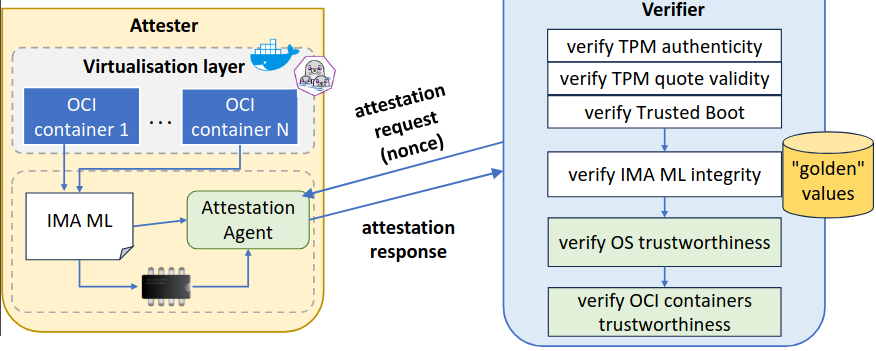
\includegraphics[width=0.6\textwidth]{img/container OCI .png}
  \caption{Remote attestation for OCI containers}
\end{figure}
This process works seamlessly with the container runtime and
workloads, enabling remote attestation of both the host and
containers. Attesting the host is essential since it's the base layer;
if compromised, the integrity of all containers would be at risk. Once
the host is verified, we can choose to attest containers individually
or in specific groups, depending on our needs.

The architecture includes a hardware root of trust, an attestation
agent, and a virtualization layer tailored for container environments.
When any operation is measured, it’s labeled to indicate where it was
executed—either on the host or within a specific container. This
labeling ensures clarity, as operations that appear to be running
inside containers are actually executed on the host OS.

During attestation, the verifier sends a request containing a nonce,
and the platform responds with the measurement list, nonce, PCR
values, and a TPM-signed response. The process first involves checking
that the TPM’s digital signature matches the expected node
certificate. Then, we verify the TPM quote to confirm that the
signature aligns with the PCR values and that the PCRs tied to trusted
boot contain the expected values. Following this, we assess the IMA
measurement list for both the host and containers, comparing these
against known good values, or “golden” values.

\subsubsection{Implementation}

The implementation of RA for OCI containers extends IMA template
called \texttt{ima-dep-cgn}.
This template is designed to enhance the attestation process by
addressing the following key aspects:

\begin{itemize}
    \item \textbf{Dependencies:} The template helps to determine
      whether an entry belongs to the host or to a specific container,
      establishing a clear relationship between the two.
    \item \textbf{Control-Group Name:} This identifier specifies the
      particular container associated with the entry, allowing for
      accurate tracking and management.
    \item \textbf{Template Hash:} The digest for the entry is
      calculated using an algorithm other than SHA-1, with options
      such as SHA-256 or SHA-512, ensuring a more secure and robust
      hashing process.
\end{itemize}

\begin{figure}[H]
  \centering
  \includegraphics[width=0.6\textwidth]{img/container OCI
  implementation.png}
  \caption{Implementation of remote attestation for OCI containers}
\end{figure}

\subsection{Credentials chain of trust}
Another main issue is privacy: in fact, the TPM is signing the
measurements with its own private key, and if you move that machine to
different environments you will be able to trace that it is always the
same machine because the signature will be created always with the
same public key. So we would like to create a chain of credentials
 that are trusted but that protect privacy.

 In the end we would like to move from TPM vendor issued keys, which
 are traceable, to a customer-usable certificate. There's also a
 specific standard for this, IEEE 802.1AR, which is a standard for 
securing a device identity using a TPM, whicle also allowing zero
touch management of a platform, but in order to do that you need the
identity of that element, a trusted identity

Inside the TPM, there's a Endorsement Key (EK) which is unique to each
TPM, with the respestive EK certificate issued by the TPM vendor(this
is also a proof that the component is genuine). We dont use that to
avoid tracing by the vendor. Instead, because the TPM is usually
enbedded on another device, the manifacturer additionally provides a
IDevID based on the EK and the TPM vendor certificate, which, top
maintain chain of trust, is linked to the TPM vendor one and cannot be
moved to another machine. This IDevID is still inside the TMP, but we
dont use that either to avoid tracing by the vendor. Instead, in the
moment in which you deploy this machine inside your IT infrastructure
another key pair whose certificate depends on the IDevID and the OEM
certificate is created. This is the local device identifier (LDevID)
which is based on the IDevID and the OEM certificate, and one can use
this key to perform operations without being traced by the vendor,
while still demostrating that it's genuine.

\begin{figure}[H]
  \centering
  \includegraphics[width=0.6\textwidth]{img/credential chain of
  trust.png}
  \caption{Credentials chain of trust}
\end{figure}

Let's go through how the sequence for creating or activating a
credential works. We have three main parts: the TPM itself, the host
platform that contains the TPM, and an external certification
authority. The process begins with the host platform asking the TPM to
create a new key. This applies to any keys created after the
endorsement key, like for IDevIDs or LDevIDs. The TPM responds with
the new key, providing only the public part.

Next, the host platform requests a certificate for this new key, and
to prove its legitimacy, it includes its TPM endorsement credential.
This credential demonstrates that the key request is coming from a
trusted machine. The certification authority then provides a
certificate for the new key, encrypting it with the TPM's endorsement
key. This encryption serves as proof of possession since only the TPM
that holds the endorsement key can decrypt it.

The host platform then instructs the TPM to decrypt the certificate
and verify that it indeed certifies the new key. Once decrypted, the
certificate is confirmed to be tied to the same TPM that holds the
endorsement key, establishing a genuine pairing. Now, we have a new
key that’s verified and securely linked to the same TPM, ensuring its
authenticity and security.

\begin{figure}[H]
  \centering
  \includegraphics[width=0.6\textwidth]{img/TPM credential
  activation.png}
  \caption{The TPM credential activation process}
\end{figure}

\subsubsection{TPM Basic Authorization Mechanism}

The TPM implements a basic authorization mechanism designed to ensure
secure command execution and object usage. 

The mechanisms available are:
\begin{itemize}
  \item \textbf{Direct Password-Based Authorization:} The TPM
    supports direct password-based authorization for executing
    single commands, enhancing security by requiring valid
    credentials.

  \item \textbf{Password-Based HMAC:} Commands and responses are
    authenticated using a password-based Hash-based Message
    Authentication Code (HMAC), ensuring the integrity and
    authenticity of the communication.  The mechanism utilizes both
    caller\_nonce and TPM\_nonce values to prevent replay attacks,
    ensuring that each command and response pair is unique and
    cannot be reused maliciously.
\end{itemize}

    
But the TPM is aware of various platform states and can be configured
to enforce specific policies regarding object usage, including:
\begin{itemize}
  \item \textbf{PCR Value Dependency:} Object usage can be
    restricted based on the values of selected Platform
    Configuration Registers (PCRs), ensuring that operations are
    only performed when the platform is in a trusted state.

  \item \textbf{Time-Based Restrictions:} The TPM can prevent
    object usage after a specified time, enhancing security by
    limiting the validity of operations to a defined time
    window.

  \item \textbf{Multi-Entity Authorization:} Usage of certain
    objects may require authorization from multiple entities,
    such as key holders, ensuring that a consensus is reached
    before critical operations are performed.
\end{itemize}

\subsection{Trust perimeter and attestation considerations}
Now that we have a functioning TPM and certificates for various keys,
there’s a critical issue around trust that we need to address,
specifically concerning when and how to perform attestation. Many
market solutions perform attestation when a software component is
installed. If the component's hash doesn’t match the expected value,
the installation (or in a cloud context, the download) is blocked. At
this stage, the signature from the developer is often verified.
Additionally, attestation may be conducted at load time, when the
component is loaded into memory for execution. This approach ensures
that components are measured at runtime.

However, the concept of "executable" is nuanced. For compiled
binaries, attestation is straightforward: we can measure the binary’s
hash. But for interpreted languages like Python, the executable is
actually the interpreter, while the script itself becomes an input to
the interpreter, creating challenges for accurate measurement. In
these cases, measurements must extend beyond the interpreter to the
script or input itself, if it exists as a file.

Moreover, even if a verified binary is running, its behavior might be
influenced by configuration files. For instance, an application like
IP tables reads configurations from files that can be modified during
runtime. Therefore, it’s crucial to monitor configuration files in
addition to binaries. Generally, attestation systems like IMA focus on
the file name for efficiency, but this can lead to issues if the file
contents change without a name change. To account for modifications,
attributes like the last modification date should also be considered.

The challenge intensifies with applications that store configurations
in memory rather than on disk, as is common with routers, switches,
and some firewalls. These devices are often configured through
protocols like SNMP or netconf, which send UDP packets containing
configuration data. Such configurations reside in memory, making
disk-based attestation approaches ineffective. Hewlett-Packard, for
instance, has implemented custom firmware for certain routers that can
attest to specific memory regions where routing and filtering tables
reside. This approach allows for memory-based attestation by hashing
designated memory segments, but it requires that these memory
addresses remain constant to avoid issues like memory randomization.

For attestation to be complete, measurements need to be compared
against "golden" or expected values. This becomes complex for
in-memory configurations, as they vary over time. Here, the network or
security management system becomes essential for providing the current
expected values. Such integration allows the attestation system to
verify in-memory configurations dynamically, rather than relying on
static, file-based measurements.

This approach to attestation is increasingly critical for audit and
forensic purposes. When an incident occurs, attestation provides a way
to verify the system’s state at the time, allowing us to determine
whether an incident was caused by a design flaw or a security breach.
This capability is essential in areas like autonomous vehicles, where
accidents might involve significant legal or ethical implications. By
attesting to the platform state, network path, and specific functions
at any given time, attestation can support not only regular audits but
also forensic investigations, helping identify the root cause of
failures and assigning accountability.

In addition to software attestation, there’s an emerging field called
network path attestation. This aims to verify the exact path network
packets took across routers, particularly in sensitive international
contexts. Ensuring that packets didn’t pass through unauthorized
regions, such as certain countries, could be essential in
security-sensitive scenarios. This opens new avenues for research and
potential thesis topics, particularly for those interested in
enhancing trust and accountability in modern, distributed networks.

In summary, attestation serves as a foundation for verifying what was
executed and how it was configured, enabling effective auditing and
forensic analysis. This capability is indispensable for confirming
software integrity, assessing system states, and potentially informing
legal or corrective actions when failures or breaches occur.

\subsection{SHIELD project}
To illustrate how attestation can support practical applications,
let's look at an example from a European project we participated in,
which focused on "security as a service." In this approach, security
functions are deployed as needed over the network infrastructure used
by the user. This is typically achieved by creating and deploying
virtualized network security functions (VNSFs) where they are needed.
In our project, we used a trust monitor to perform attestation on the
infrastructure, which was primarily software-based.

In the setup, the trust monitor worked in conjunction with an NFV
(Network Function Virtualization) infrastructure. This infrastructure,
managed by an orchestrator, was the target for deploying various
security functions. Additionally, a store provided network security
functions as software objects, while a security dashboard displayed
the system's status. If any security misconfiguration or integrity
issue was detected, there was also a reaction mechanism to address it.
This framework was part of the Shield Horizon 2020 project, an
NFV-based security infrastructure aimed at monitoring, enforcing
security actions and reactions, and using remote attestation to verify
the integrity of the entire infrastructure.

The trust monitor received two key inputs. The first input came from
the infrastructure itself, allowing the monitor to assess whether the
system was correctly configured and running the expected components.
This involved periodic requests to each component for attestation
results, ensuring that the trust monitor could check each component’s
current measurements. The second input came from the VNSF store,
providing “golden” measurements—known values for expected
configurations and software hashes, which serve as benchmarks for
verifying each component's integrity.

When there was a mismatch between a component's actual measurement and
the golden measurement from the store, an alert was triggered. This
alarm was then analyzed, allowing the system to identify what went
wrong and initiate appropriate remediation actions. Through this
combination of measurements and golden benchmarks, the trust monitor
maintained a secure infrastructure by continuously verifying the
integrity and correct configuration of deployed security functions.

\begin{figure}[H]
  \centering
  \includegraphics[width=0.6\textwidth]{img/SHIELD project.png}
  \caption{SHIELD project}
\end{figure}

\subsubsection{Golden value creation}
Let's begin with creating the "golden values." Here, we have the store
of network security functions. When the trust monitor starts, it will
request the security manifest. Every piece of software comes with a
manifest, which, among other things, specifies hash values. If a
virtualized network security function (VNSF) consists of multiple
components, the manifest includes a hash for each part.

The trust monitor retrieves the VNSF's security manifest, extracting
the measurements for each component. If a particular component's hash
is already in the database (perhaps because it's used by another
VNSF), the trust monitor will skip it. However, if the measurement is
new—meaning this component hasn't appeared in any other VNSF yet—it
will add this hash to the whitelist database. This list, also known as
a "whitelist" or "accept list," identifies the components that are
authorized to run on the system.

\begin{figure}[H]
  \centering
  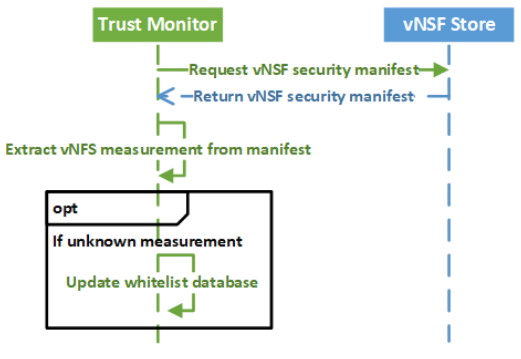
\includegraphics[width=0.4\textwidth]{img/shield golden value.png}
  \caption{Golden value creation}
\end{figure}

\subsubsection{Initial deployment of a security function}
When deploying a security function, the orchestrator initiates the
process by requesting the trust monitor to verify the state of the
host, or "middle box," where the function will run. Before placing a
virtual network security function (VNSF) on a host, it’s essential to
confirm that the host system is in a secure and trusted state. This
includes checking that the operating system, Docker container runtime,
and boot process are intact and secure.

To do this, the trust monitor initiates a remote attestation by
sending a nonce to the target host. In response, the host provides a
TPM quote and event log as proof of its current integrity. If the
attestation results match the expected, secure values, the trust
monitor returns a "success" message to the orchestrator. This
validation allows the orchestrator to include the middle box in the
list of authorized nodes for deployment.

However, if the attestation fails to verify, the trust monitor returns
a "failure" message, and the host is excluded from further
orchestration. An alarm is also triggered, notifying the security
manager to investigate the physical node's status. Until resolved, the
node remains isolated and is not considered for any subsequent
deployment steps.
\begin{figure}[H]
  \centering
  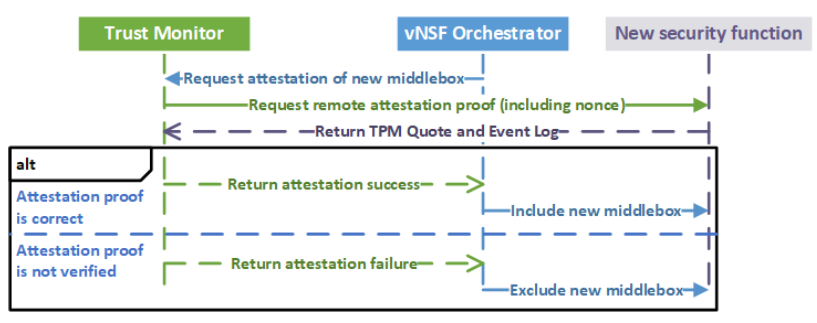
\includegraphics[width=0.6\textwidth]{img/shield deployment.png}
  \caption{Initial deployment of a security function}
\end{figure}

\subsubsection{Periodic attestation of security functions}
Next, there is the process of periodic attestation, which the trust
monitor performs automatically at intervals determined by the security
manager. These intervals are typically based on the expected speed of
potential attacks and are usually set in the range of minutes—such as
every 10, 30, or 60 seconds—rather than hours.

For each cycle, the trust monitor requests the current network state
from the orchestrator, which identifies the specific nodes currently
involved in security functions. This ensures that only relevant nodes
are attested, rather than the entire network, focusing on the nodes
that a particular customer or application may be using (e.g., nodes 2,
7, and 35).

With the list of active nodes, the trust monitor requests a remote
attestation proof from each middle box in this subset. Each node
provides a TPM quote and event log as proof of its current integrity.
If the attestation result is positive, the network continues to
operate as normal. However, if a failure is detected, the trust
monitor triggers an alert through the security dashboard, notifying
the operator of a potential issue with the affected node. 

At this point, the operator has the option to manually intervene, such
as by terminating, isolating, or reconfiguring the problematic node.
While automated responses could be implemented with AI, this project
favors a "human-in-the-loop" approach, leaving the final decision to
the operator after receiving the alert.

\begin{figure}[H]
  \centering
  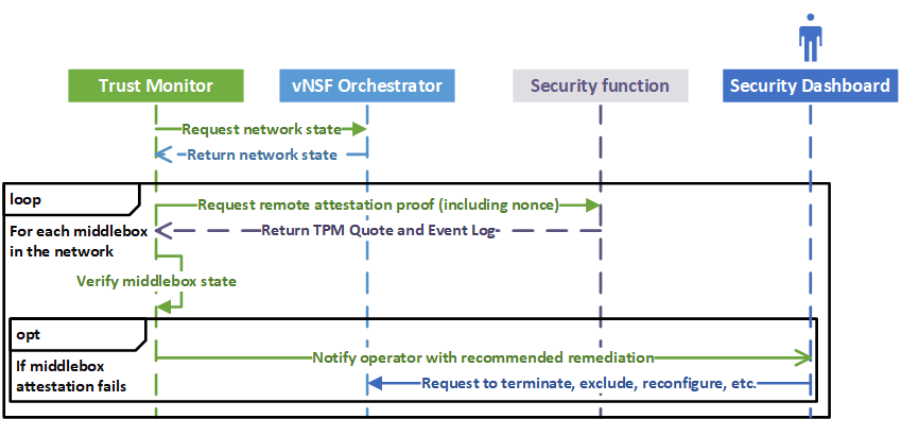
\includegraphics[width=0.7\textwidth]{img/shield periodic attestation.png}
  \caption{Periodic attestation of security functions}
\end{figure}

\section{Keylime}

Keylime is an open-source remote attestation project hosted at the
Cloud-Native Computing Foundation (CNCF) that is designed with a focus
on cloud-oriented environments. It leverages a physical TPM to create
a highly scalable RA framework with a straightforward architecture.

Keylime includes several key features: remote boot attestation, which
ensures the integrity of the boot process by verifying the platform's
state at boot time; Linux IMA support, allowing for periodic runtime
attestation through IMA to verify system integrity during operation;
registration of multiple agents to a central verifier, enhancing
flexibility and scalability in attestation processes, in fact, an
agent is the piece of software that you need on the node to create the
attestation port, m.t. one can have as much as needed ; and a
additional certificate infrastructure to facilitate secure
communications and verifications within the framework. Why it's part
of the standard? Because at least initially, Keylime gave to each
agent also a public key certificate in order to perform operations
like signatures, but it's rarely used nowadays.

\begin{figure}[H]
  \centering
  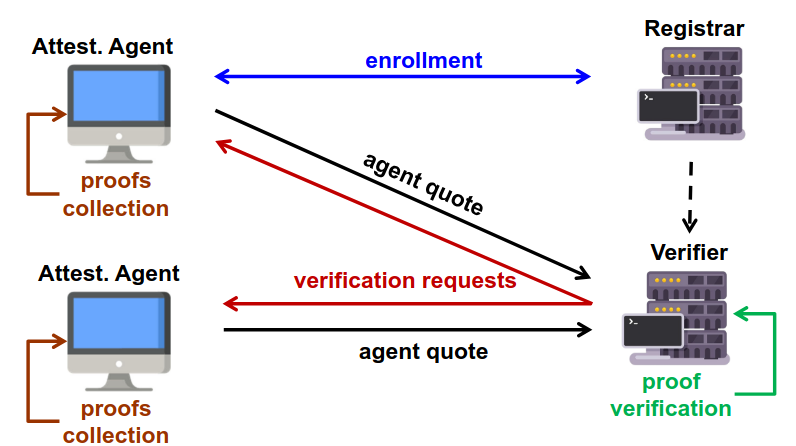
\includegraphics[width=0.6\textwidth]{img/keylime schema.png}
  \caption{Keylime schema}
\end{figure}

\subsection{Keylime Structure}

The Keylime framework is composed of several key components that work
together to enable remote attestation of nodes. 

The \textbf{attester agent} is a software component installed on each
node that needs to respond to remote attestation requests. Its primary
function is to retrieve the TPM quote, which includes the PCR values
signed by the TPM’s internal key. In addition to the quote, the agent
gathers other necessary data, such as the IMA measurement list for PCR
10. Optionally, the agent can also listen for revocation messages if
certificate-based attestation is used and a certificate has been
revoked.

The \textbf{registrar} manages the enrollment of attester agents. When
a node with an agent is deployed, it must be registered with the
registrar, which assigns it a unique user identifier. The registrar
also handles the management of agent keys, including the agent’s
signing key and the endorsement keys stored in the TPM.

The \textbf{verifier} is responsible for attesting the nodes by
communicating with the attester agents. It requests and validates the
TPM quotes and can send revocation messages if an agent is determined
to be in an untrusted state, especially in cases where certificate
revocation is utilized.

Finally, the \textbf{tenant} represents the entity that owns or
manages a specific part of the infrastructure. It provides a unified
interface for managing the agents across the infrastructure, enabling
consistent and centralized management of attestation operations.

\subsection{General Schema}
This is the schema we are discussing. In our network, we have two
nodes that require attestation. Each of these nodes needs to run an
attestation agent. Additionally, there will be a machine designated as
the registrar and another as the verifier. While it's not mandatory to
have them separate, they are distinct processes. You can run both the
registrar and the verifier on the same machine.

The registrar is responsible for enrollment. When an agent is
deployed, it attempts to enroll itself, and the registrar notifies the
verifier of this new registration, instructing it to perform periodic
attestations for that node. The verifier will then regularly send
verification requests to the various agents. Each agent gathers the
necessary proofs, such as the PCR values and, if IMA is enabled, the
IMA measurement list. It sends a quote containing all required
information back to the verifier. This process is repeated for each
node in the network.

While this architecture functions well, it does have a vulnerability:
the presence of a centralized verification point creates a single
point of failure. If the node containing the registrar or verifier is
compromised or subjected to a denial-of-service attack, we lose
visibility into the network's state. A possible approach to mitigate 
this is to adopt a decentralized architecture, and one of the
possibilities that is being discussed is to use a blockchain.

In the event of a critical node being compromised, there would need to
be a protocol to notify administrators to deploy a replacement node.
This concept of a self-healing network is significant, as it allows
the network to recover autonomously from attacks by excluding
malicious nodes.

Regarding the chain of trust, you can choose to utilize an endorsement
key or other keys as part of this framework. While the chain of trust
is not strictly required, a minimum setup for a node with a TPM
includes the endorsement key, which is always present. If privacy is a
concern, the chain of trust can be established with identifiers like
the IDevID and LDevID.

At last, each time a quote is received, it will be verified against
the golden measurements to ensure integrity.

\subsection{Remote Attestation Procedures – RATS}

The Remote Attestation Procedures (RATS) were proposed by the Internet
Engineering Task Force (IETF) to enhance support for different
platforms during the load time. RATS defines various actors involved
in the remote attestation procedures, including the Attester, Relying
Party, Verifier, Relying Party Owner, Verifier Owner, Endorser, and
Reference Value Provider. The definition of all this roles sure helps
in environments such as the cloud.

Additionally, RATS specifies several topological patterns, such as the
\textbf{Background Check} and the \textbf{Passport} Model, to organize
the interactions among these actors. The framework is documented in
RFC-9334, titled "RATS Architecture," which lays the foundation for
the remote attestation process. Numerous other RFC drafts are
currently in progress, focusing on various aspects such as data
formats, procedures, and attestation models to further develop the
RATS framework.

\subsubsection{Interaction schema}

This diagram in figure \ref{fig:rats} outlines the schema of
interactions, with the verifier as the central component. The
\textbf{verifier}'s primary function is to receive quotes and
determine their validity—whether they are good or bad. To make this
determination, the verifier collects evidence from the
\textbf{attesters}, including quotes, mailing lists, signed PCRs, and
other relevant data. It then provides attestation results to a relying
party, which is an entity that trusts the verifier to conduct this
verification.

However, this is just the basic setup. To enhance the process, we
introduce the concept of the endorser. An endorser is an entity that
designates the correct elements to be verified within the system. For
example, if you've purchased a component from another company, you
would need to measure it, but the measurements must be supplied by
that vendor.

The verifier has an owner responsible for setting up the appraisal
policy for the evidence. This is particularly important for software
components, as you may have both current and legacy versions in your
network. Questions arise regarding which versions to accept: Is it
only the latest version, or are older versions accepted as well? You might
categorize versions based on their status—some may lack functionality,
while others could have critical bugs or security vulnerabilities.
Policies should be established to define acceptable conditions for
older versions, allowing acceptance of those that only have missing
functionality but rejecting those with known issues.

In addition to the verifier owner, there is the relying party owner,
who must decide the appropriate course of action based on the
attestation results. They determine whether the results are acceptable
and assess the severity of any issues identified.

\begin{figure}[H]
  \centering
  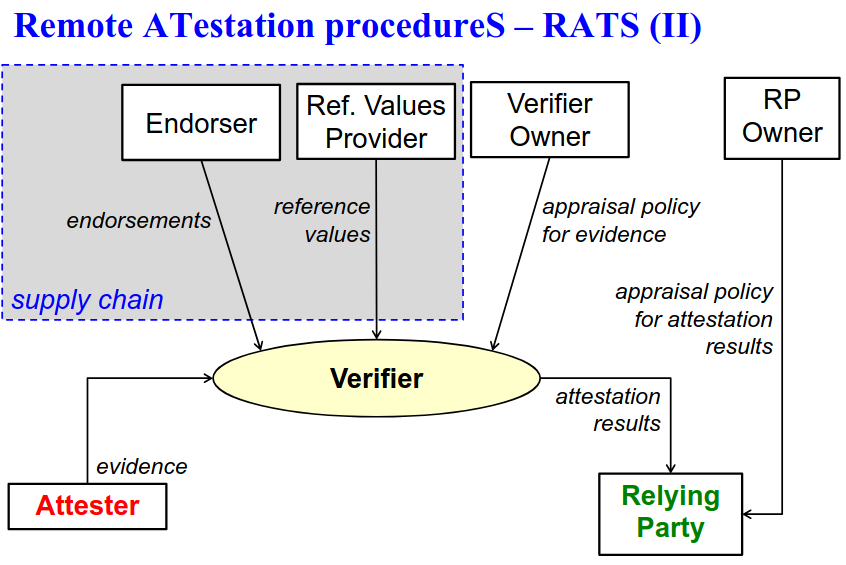
\includegraphics[width=0.6\textwidth]{img/RATS.png}
  \label{fig:rats}
  \caption{Remote Attestation Procedures (RATS)}
\end{figure}

\subsubsection{RATS – Main Roles}

Let's go now in details by providing a formal definition of the main
actors.

The \textbf{Attester} is responsible for generating evidence when
attestation is needed, typically at the request of the Relying Party.
This evidence is essential for accessing services, such as those that
utilize OAuth for authentication. This is important because even if a
node has the correct token it may be infected.

The \textbf{Verifier} plays a critical role in comparing the evidence
provided by the Attester against predefined reference values, applying
an appraisal policy in the process. It also utilizes endorsements to
identify valid attesters, ensuring that the attestation is credible.

Finally, the \textbf{Relying Party} evaluates the attestation results
based on its specific policy, known as the Relying Party Policy. It is
important to note that the Relying Party and the Verifier may be part
of the same service, streamlining the attestation process.

\subsubsection{Attestation Models}

There are two main models for running attestation: the background
check model and the passport model.

\paragraph{Background Check Model}: In this model, the attester
provides evidence, which is then passed on to the relying party.
However, the relying party cannot evaluate the evidence on its own, so
it sends the evidence to a verifier. The verifier reviews the evidence
and sends back an attestation result to the relying party. This is
similar to a background check, where an external authority is
consulted to verify someone’s status. For instance, when you go to buy
a firearm, the shop (acting as the relying party) contacts law
enforcement (the verifier) to confirm if you’re eligible to make the
purchase. Similarly, when a company hires an employee, it might
conduct a background check, examining the candidate’s online history
to ensure they align with company values. Many companies now require
applicants to share their social media profiles for such checks. In
both cases, external evidence is checked by an independent verifier on
behalf of the relying party.

\paragraph{Passport Model}: In this model, the attester creates
evidence and submits it directly to the verifier. The verifier then
reviews this evidence and issues an attestation result back to the
attester, who can present it to the relying party. It’s like
presenting a passport when traveling: instead of the relying party
(e.g., a border control officer) having to verify your identity
independently, you present a pre-verified document. This model allows
the attester to proactively acquire verification from the verifier,
making it readily available for the relying party. Using the previous
example, imagine obtaining a certificate of good standing from the
police before entering a store. This way, you’re pre-approved, and the
store doesn’t need to conduct further checks.

In both models, the final attestation result is provided to the
relying party, which relies on this verification to establish security
and trust.


\begin{figure}[H]
  \centering
  \includegraphics[width=0.6\textwidth]{img/RATS attestation
  procedure.png}
  \caption{RATS attestation procedure}
\end{figure}

\section{Veraison (VERificAtIon of atteStatiON)}

Nowadays, one of the main problems in attestation is that every
companby is developing its own solution, and this is a problem because
there's no interoperability. We would like to have a generic verifier,
which can be used with any kind of attestation produced by any kind of
company.

Veraison is an open-source project designed to enhance consistency for
Verification Services in the realm of remote attestation. It
implements various standards and provides a set of libraries that
allow for extensive customizations.

Originally generated by ARM's Advanced Technology Group (ATG),
Veraison was later adopted by the Confidential Computing Consortium
within the Linux Foundation. It supports a variety of architectures
and RoT implementations, making it a versatile
solution in the field of attestation.

While Veraison does not offer a standard agent implementation, it
features a flexible structure for evidence provisioning. Its high
customizability enables users to select only the necessary features
for their applications, facilitating the easy development of custom
functionalities tailored to specific requirements.

\subsection{Veraison Architecture}
The architecture of Veraison is shown in figure
\ref{fig:veraison-architecture}. The components highlighted in blue
are managed by Verizon Trusted Services. Verizon handles several
plugins to facilitate attestation, including a handler for
endorsements that allows connection to any endorser of your choice, as
well as a handler for evidence. Within the provisioning process, there
is a plugin manager for coordinating these plugins. Verification
occurs outside of this managed area, and there is also a key-value
store for maintaining relevant information. 
\begin{figure}[H]
  \centering
  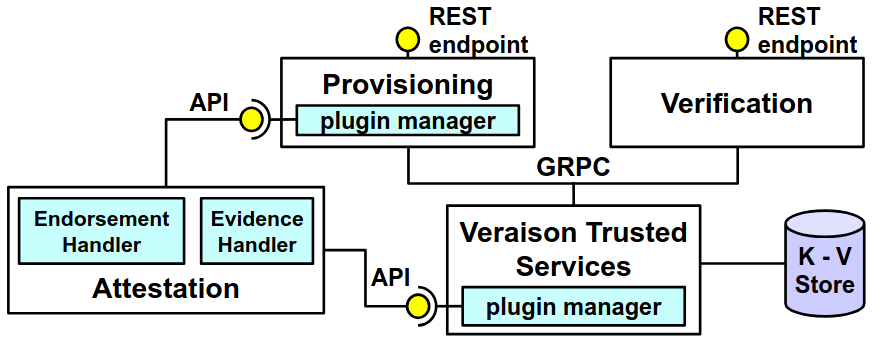
\includegraphics[width=0.6\textwidth]{img/veraison architecture.png}
  \label{fig:veraison-architecture}
  \caption{Veraison architecture}
\end{figure}

\subsection{Verification}
Verification is at the core of Verizon's functionality, and it
involves a complex, multi-step process. Upon receiving a request, the
handler performs the verification steps, all of which are integral to
Verizon’s operations. This includes support for different media types,
which can each be processed in a customized way. The process also
involves establishing trust anchors—root authorities that certify the
TPM or your own root of trust. Key stages include handling claims,
endorsements, validation, appraisal, and signatures, among other
tasks.

\begin{figure}[H]
  \centering
  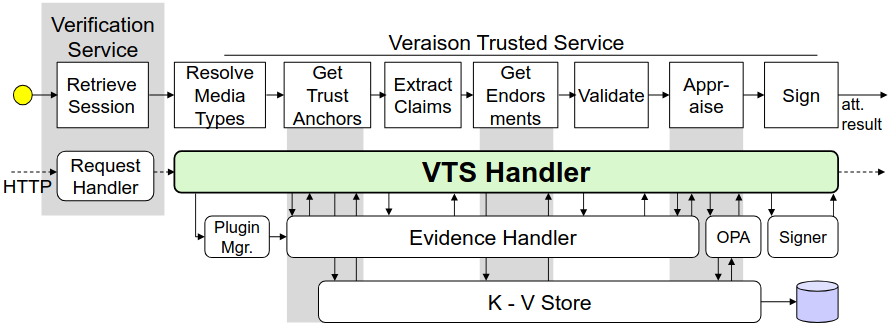
\includegraphics[width=0.6\textwidth]{img/verizon verification.png}
  \caption{Veraison verification}
\end{figure}
\subsection{Data formats}

Data formats are essential for achieving interoperability in
attestation. Verizon’s architecture natively supports ingestion and
generation of various attestation formats.

\paragraph{Entity Attestation Tokens (EAT)}  
The attestation results are formatted as Entity Attestation Tokens,
which can be encoded in CBOR or JSON. EAT is used as a standardized
format for representing evidence, especially within the PSA (Platform
Security Architecture) ecosystem—a security certification schema
designed for IoT devices.

\paragraph{Evidence Formats}  
Evidence can be presented in multiple formats, including:
\begin{itemize}
    \item \textbf{PSA-EAT} — Developed under the PSA framework,
      primarily for IoT security.
    \item \textbf{CCA (Confidential Compute Architecture)} — The
      format used by ARM for secure compute environments.
    \item \textbf{TPM and DICE} — Trusted Computing Group (TCG)
      standards, where TPM is a longstanding standard, while DICE is
      designed for embedded and IoT systems.
    \item \textbf{Amazon Nitro} — Amazon’s format for creating
      evidence within secure enclaves.
\end{itemize}

\paragraph{Endorsements and Reference Values}  
Endorsement and reference values are represented using CORIM (Concise
Reference Integrity Measurement). CORIM includes:
\begin{itemize}
    \item \textbf{COMID} for hardware and firmware modules,
    \item \textbf{COSWID} for software components, and
    \item \textbf{COBOM} (Concise Bill of Materials) for hardware,
      software, and cryptographic inventories.
\end{itemize}
The bill of materials is essential in security frameworks, such as
NIST’s, where inventory management is a primary phase of security
planning. Each element's hardware, software, and cryptographic
components are listed to support system transparency.

\paragraph{Appraisal Policy for Evidence}  
For appraising evidence against policies, Open Policy Agent (OPA)
provides an open-source solution where policies can be defined and
applied. This enables a comparison between attestation results and the
established policy.

\paragraph{Attestation Result Formats}  
Attestation results can be formatted in EAR for general attestation
and R4C for secure interactions, offering flexibility in secure
communication.

This broad range of formats ensures compatibility across platforms,
though the variety also introduces significant complexity.

\section{Device Identity Composition Engine (DICE)}
So, insofar we discussed the attestation as was originally conceived,
that is using a hardware root of trust implemented with the TPM. That
is perfectly fine, but it's a rather complex solution, because TPM is
a complex object that needs either to be implemented as a physical
chip, or if it is in firmware, it's a large component. There are some
alternatives being proposed for systems that cannot have additional
hardware, and even running large portions of firmware is not suitable
for them. Typically, they are internet of things or embedded systems
with limited computational capacity.

The Trusted Computing Group developed the Device Identifier
Composition Engine (DICE) to establish secure device identities,
focusing on identifying each layer of the device through cryptographic
keys. DICE’s approach centers on the Compound Device Identifier (CDI),
a unique secret value, usually a private key, generated by applying a
one-way cryptographic hash to combine a secret for the current layer
and a measurement of the next.

DICE’s process involves layered identity verification. Each layer,
beginning with firmware, is measured and linked to a unique key. When
a new layer is initialized, DICE generates a new key based on the
prior layer’s key and the measurement of the upcoming layer. This
ensures that any tampering at one layer disrupts the chain, as the
altered measurement would produce a mismatched key.

At the base of this chain is the Unique Device Secret (UDS), a
distinct and randomly generated secret that initializes the first CDI
value. The UDS is statistically unique, ensuring it cannot correlate
with UDS values on other devices. In practice, this may be created
using a physically unclonable function (PUF) to generate a unique
random value specific to the device.

Each CDI is recalculated upon reboot, depending on the device’s static
software state. If the software remains unchanged, the same keys are
generated; otherwise, new keys indicate tampering. Verification
against a public key certificate confirms the integrity of the
system—any unauthorized software changes disrupt this chain of trust,
invalidating the certification.

\subsection{DICE Layered Architecture}

The DICE architecture begins at the boot stage, forming the
foundational layer for secure identity. The DICE layer alone has
access to the UDS, a crucial element for establishing trust, and
calculates the initial TCI for layer zero by hashing the software code
of this layer. Using a one-way function (hash), the DICE layer then
generates a unique key for the next layer in the boot sequence.

Each subsequent layer repeats this process: it measures the software
of the following layer, applies a hash function, and combines it with
the current CDI to generate a new CDI for the next layer. This
recursive measurement and key generation process continues across
layers, linking each layer’s identity to its software integrity.
Typically, only a few layers are involved, but the approach allows for
as many layers as needed.

In essence, these keys are dynamically generated based on the software
at each layer. Identical keys are recreated only if the software at
each layer remains unchanged, thereby ensuring that any modification
to a layer disrupts the integrity chain.

\begin{figure}[H]
  \centering
  \includegraphics[width=0.6\textwidth]{img/dice layered
  architecture.png}
  \caption{DICE layer architecture}
\end{figure}

\subsection{Dice keys and certificates}
In the DICE architecture, each layer can have multiple keys and
certificates, expanding beyond the initial key generated by the DICE
layer for the first Compound Device Identifier (CDI). Starting from
layer 0, a key derivation or key generation function produces
additional keys for that layer, with each subsequent layer performing
the same process. Rather than using the CDI directly, these derived
keys serve in cryptographic operations.

Each layer may include an Embedded Certification Authority (ECA),
which issues certificates for attestation or identity verification.
This ECA is designed to sign only data it generates, preventing
potential risks associated with signing external data. There are three
primary types of keys:

\begin{itemize}
  \item ECA Key: Used to issue certificates for keys generated in the
    current or next layer, eliminating the need for an external
    certification authority—a practical approach for embedded or IoT
    devices.
  \item Attestation Key: Used to sign attestation evidence, ensuring
    integrity in reporting the device's state.
  \item Identity Key: Used exclusively for identity verification
    through challenge-response protocols, maintaining secure device
    authentication.
\end{itemize}

This layered approach allows for distinct roles for each key, although
a single versatile certification authority could be employed for
simplicity.

\begin{figure}[H]
  \centering
  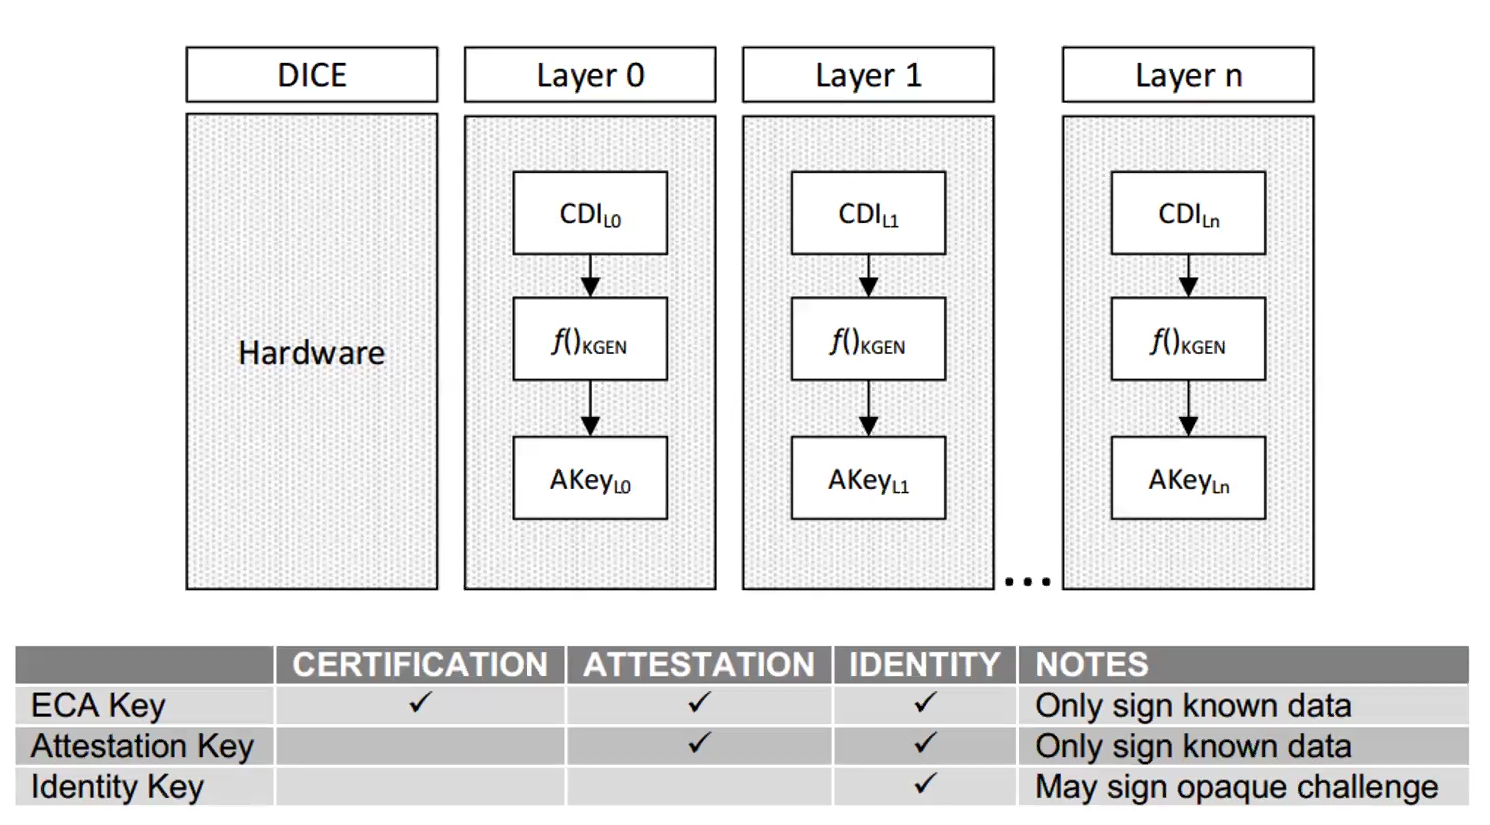
\includegraphics[width=0.6\textwidth]{img/dice keycert.png}
  \caption{DICE keys and certificates}
\end{figure}

\subsection{Dice layered certification}
\begin{boxH}
  Each layer in the DICE framework can act as an ECA, establishing a
  certification hierarchy rooted in the manufacturer’s root CA. 
\end{boxH}
Each ECA can produce two different types of certificate.
The device manufacturer provides this root CA, which issues the first
certificate for the CDI (Compound Device Identifier) of the DICE
layer. Since the DICE layer is meant to be immutable, except when a
firmware update is performed, this initial certificate remains
constant and can be externally verified as a marker of platform
authenticity.
The ECAs in subsequent layers issue certificates (the second kind)
that represent the device's identity and attestation status. 

Each certificate includes specific X.509 v3 extensions crucial to DICE
architecture compliance, namely `DICE PCB Info` and `DiceTcbInfo`.
These extensions contain vital identification and measurement data
required for device authentication and security.

\begin{itemize}
    \item \textbf{DiceTcbInfo Extension}: Each certificate must
      include the `DiceTcbInfo` extension with OID:
    \[
    2.23.133.5.4.1 =
    \text{joint-iso-itu(2).international-org(23).tcg(133).tcg-platformClass(5).dice(4).TcbInfo(1)}
    \]
    This extension provides a SEQUENCE of information specific to the
    device’s target level, containing:
    \begin{itemize}
        \item \textbf{Names}: Identification fields such as
          \textit{vendor, model, and layer}.
        \item \textbf{Measurements}: Versioning and security
          attributes, such as \textit{version, security version number
          (svn)}, and \textit{fwidlist} (a list of firmware IDs, each
          represented by a \textit{hash algorithm and digest}).
    \end{itemize}
    
\end{itemize}


The certificate, therefore, holds key information about the platform,
without revealing its full details. Instead of explicitly naming
firmware, it provides a digest. This digest allows anyone with the
necessary knowledge to validate the platform’s firmware identity,
while keeping exact firmware information private.
\subsection{Dice on RISC-V}
The professor recenly completed another project on September 30 and
are now preparing to launch the next phase. This project involved
implementing DICE on a RISC-V platform equipped with a hardware
cryptography accelerator. In this setup, layer 0 contains the Compound
Device Identifier (CDI), also referred to as the device root key,
which is accompanied by a root key certificate issued by the platform
manufacturer.

For this solution, we integrated with Keystone, a system where the
security monitor serves as the foundational layer. Here, the device
root key signs the key of the Embedded Certification Authority (CA)
specifically for the security monitor. The security monitor, in turn,
generates an initial attestation key and issues the initial device ID
certificate for the device, establishing a certified identity for the
device.

In Keystone’s architecture, trusted enclaves are established, isolated
from the untrusted parts of the system. Each enclave can generate a
local device identifier with its own certificate, signed by the
previous layer, along with a local attestation key. Embedded CAs are
not necessary within each enclave since they do not generate additional
keys. Importantly, this entire chain of trust originates from the
manufacturer’s root certificate, which could pose privacy concerns if
used directly in a user's system.

To address privacy, an option exists to associate a new certificate
with the device identifier of each enclave. This approach allows users
to use the same keys while issuing the public key to their own
certification authority for signing. Consequently, the root of trust
can shift from the manufacturer to the user’s chosen authority. Once
verified, this new certificate can be used exclusively.

If an attack or modification occurs in the platform, security monitor,
or enclave, the system will automatically invalidate the certificate.
Any changes in the trusted software or applications alter the generated
keys, making the certificate invalid as it would now contain a
different public key. Rather than storing keys persistently, keys are
regenerated as needed and remain bound to the executing software,
thereby reinforcing security.

\begin{figure}[H]
  \centering
  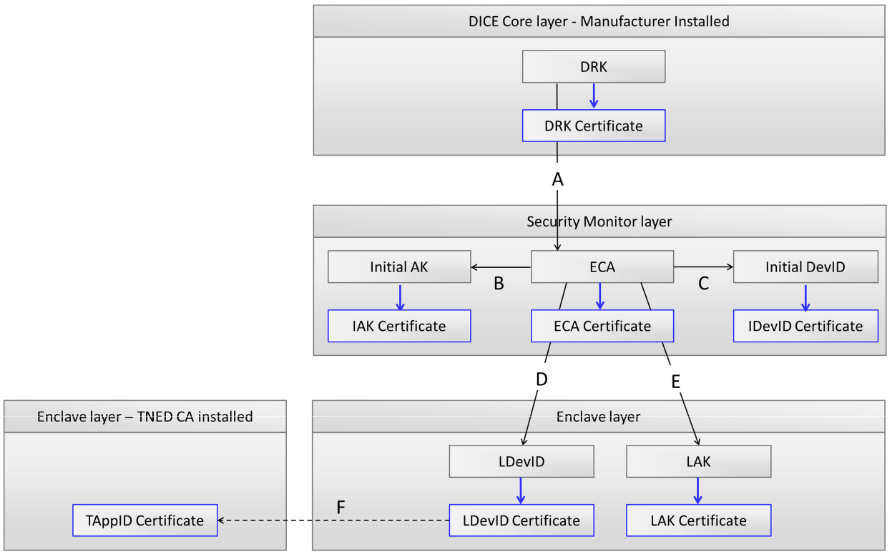
\includegraphics[width=0.6\textwidth]{img/dice riscv.png}
  \caption{DICE on RISC-V}
\end{figure}

\subsection{Open Profile for DICE}

The Open Profile for DICE is a specification from Google for
implementing DICE. In this model, each layer in the system is
equipped with two types of Compound Device Identifiers (CDIs):
\begin{itemize}
    \item \textbf{Attestation CDI} (mandatory)
    \item \textbf{Sealing CDI} (optional)
\end{itemize}

The CDI for each subsequent layer is derived using additional specific
input values, depending on the CDI type. These inputs include:
\begin{itemize}
    \item \textbf{Configuration Data:} Information regarding the
    integrity of the system.
    \item \textbf{Authority Data:} A hash representing information
    about the trusted authority used in verified boot.
    \item \textbf{Mode Decision:} The current operating mode of the
    device.
    \item \textbf{Hidden Inputs:} Values that are not disclosed in
    any certificate.
\end{itemize}

Furthermore, each layer has an Attestation keypair, which is derived
from its corresponding Attestation CDI, enabling cryptographic
attestation at each stage.

\subsection{DICE and RIOT}

RIOT (Robust Internet of Things) is Microsoft's specification for
implementing DICE. Unlike the standard DICE implementation, RIOT
utilizes a single Compound Device Identifier (CDI) for the entire
device. Key aspects of RIOT's DICE model include:

\begin{itemize}
    \item \textbf{Single CDI:} The CDI is generated by combining the
    platform's Unique Device Secret (UDS) with the measurement of the
    RIOT core, which is the only software component permitted to
    access the CDI.
    \item \textbf{Alias Keypairs for Attestation:} Each layer
    includes an Alias keypair for attestation.
    \item \textbf{Recursive Key Derivation:} Each layer \(N\) uses
    the measurement of the subsequent layer \(N+1\) to compute its
    Alias keypair. For the RIOT core, this Alias keypair is derived
    directly from the CDI.
\end{itemize}

\subsection{Cloud providers and DICE}
Let's wrap this chapter up by showing what the major cloud providers 
are doing with DICE.

\subsubsection{Google Cloud Attestation}

Google Cloud provides optional attestation for platform security, with
key capabilities supported on services such as Google Kubernetes
Engine (GKE) and Cloud Run. A central feature is binary authorization,
which includes various scans and analyses—such as vulnerability scans,
regression tests, and signing of the container image hash—to ensure
container integrity.

At deploy-time, Google Cloud enforces security controls by blocking
any container deployment lacking a valid signature. If the container
meets the specified policies, deployment is allowed, ensuring
policy-compliant security for containerized applications.

\subsubsection{Amazon Web Services Attestation and Security}

Amazon Web Services (AWS) provides several security features related
to container integrity, though not traditional attestation. AWS
Elastic Container Registry (ECR) stores container images that can be
executed, and Amazon Inspector offers scanning capabilities for these
images.

Amazon Inspector scans container images each time a new image is
pushed or a new vulnerability definition is added. An additional
feature, enhanced scanning, checks for vulnerabilities in the
operating system and within specific programming languages. Users can
specify the programming language used, allowing AWS to scan for known
vulnerabilities relevant to that language. AWS also checks service
vulnerabilities, particularly regarding network access, to enhance
container security.

\subsubsection{Amazon Web Services NITRO Attestation}

AWS provides a form of attestation through NITRO, a specific type of
enclave used for secure execution within a VM. NITRO enclaves are
isolated and constrained, only able to communicate with their parent
EC2 instance. The enclave can request attestation from the NITRO
manager to prove its integrity and request services. For example, an
enclave can ask the NITRO manager to attest its state, and the NITRO
manager can request the parent EC2 instance to sign or decrypt data on
behalf of the enclave.

The attestation process in NITRO occurs during load time, ensuring
that the correct binary is loaded into the enclave. Once the correct
binary is confirmed, runtime services are provided, and the
attestation process is no longer necessary. While attestation takes
place at runtime, it primarily verifies the initial loading of the
enclave, rather than continuous runtime checks.


\subsubsection{AWS Nitro's PCRs}

AWS Nitro utilizes PCRs intead of TPMs for various attestation
measurements. The following PCRs are defined for different components:

\begin{itemize}
    \item \textbf{PCR0 (Enclave Image File):} Measures the enclave
      image file, excluding the section data.
    \item \textbf{PCR1 (Linux Kernel and Bootstrap):} Measures the
      Linux kernel and boot RAM filesystem (ramfs) data.
    \item \textbf{PCR2 (Application):} Measures the user applications,
      excluding the boot ramfs.
    \item \textbf{PCR3 (IAM Role Assigned to the Parent):} Attestation
      succeeds only if the parent EC2 instance has the correct IAM
      role assigned.
    \item \textbf{PCR4 (Instance ID of the Parent):} Attestation
      succeeds only when the parent EC2 instance has a specific
      instance ID.
    \item \textbf{PCR8 (Enclave Image File Signing Certificate):}
      Attestation succeeds only if the enclave was booted from an
      image file signed by a specific certificate.
\end{itemize}

\subsubsection{Azure Confidential Containers}

Azure Confidential Containers provide secure deployment and
attestation of containers through the following process:

\begin{itemize}
    \item Upon container deployment, a token is generated and signed
      by the cloud node.
    \item The token is verifiable by a remote entity.
    \item The token includes information about:
    \begin{itemize}
        \item The correct deployment of the container in a Trusted
          Execution Environment (TEE).
        \item The use of a VM-based TEE.
        \item A hardware-based and attested TEE.
        \item Full guest attestation.
    \end{itemize}
    \item The solution provides additional data and code protection.
    \item There is no need for a specialized programming model or
      special management.
\end{itemize}

